\documentclass{ieeeaccess}
\usepackage{cite}
\usepackage{amsmath,amssymb,amsfonts}
\usepackage{algorithmic}
\usepackage{graphicx}
\usepackage{caption}
\usepackage{url}
\usepackage{amsmath}
\usepackage[english]{babel}
\newtheorem{theorem}{Theorem}
\newtheorem{definition}{Definition}
\usepackage{scalerel}
\newcommand\sbullet[1][.75]{\mathbin{\ThisStyle{\vcenter{\hbox{%
  \scalebox{#1}{$\SavedStyle\bullet$}}}}}%
}
\usepackage{textcomp}
\def\BibTeX{{\rm B\kern-.05em{\sc i\kern-.025em b}\kern-.08em
    T\kern-.1667em\lower.7ex\hbox{E}\kern-.125emX}}
\begin{document}
\history{Date of publication xxxx 00, 0000, date of current version xxxx 00, 0000.}
\doi{10.1109/ACCESS.2017.DOI}

\title{Anonymous provision of services via blockchain}
\author{\uppercase{Stanis\l{}aw Bara{\'n}ski} \authorrefmark{1},
\uppercase{Julian Szyma{\'n}ski\authorrefmark{1} } 
 }

\address[1]{Department of Electronic, Telecommunication and Informatics, Gdansk University of Technology, Narutowicza 11/12 Gdansk Poland (e-mail: stanislaw.baranski@pg.edu.pl, julian.szymanski@eti.pg.edu.pl}

 

\tfootnote{The work has been supported partially by the founds of Department of Computer Architecture Faculty of Electronics, Telecommunications and Informatics, Gdańsk University of Technology.}

\markboth{S. Bara{\'n}ski, J. Szyma{\'n}ski : 
Anonymous provision of services via blockchain}
{S. Bara{\'n}ski, J. Szyma{\'n}ski : 
Anonymous provision of services via blockchain}

\corresp{Corresponding author: Stanislaw Baranski (e-mail: stanislaw.baranski@pg.edu.pl).}

\begin{abstract}
Service providers like lawyers, laboratories, auditors, or banks, to provide services, require customers to submit data often associated with their personal information. This situation exposes customers to privacy risks. However, most service providers use personal information merely for logistic operations like payments and communication and could provide services anonymously if other means of logistics exist.
We propose a protocol for coordinating anonymous service provision. Our proposal uses blockchain for both anonymous payments and proofs of existence (so-called message board) and content-addressable network (e.g.~IPFS) for results delivery.
A service provider can employ our protocol to provide services without collecting personal information. Possible applications for this protocol include anonymous tests for drugs, venereal diseases, paternity, and steroids, or anonymous legal advice.
In case of dispute, either due to exceeding deadlines or providing incorrect results, the customer can disclose the whole interaction and prove to justice (police or court) the misbehaviour of the service provider.
We analyze the protocol in the context of fairness and discuss further extensions to an anonymous delivery system, payment with cash, and a decentralized conflict resolution system.
Our protocol may enable various services currently based on unacceptable trust assumptions to the service providers.
\end{abstract}

\begin{keywords}
Anonymity, blockchain, fair-exchange, physical delivery, privacy, services
\end{keywords}

\titlepgskip=-15pt

\maketitle
\section{Introduction}
Service providers (SPs) like lawyers, laboratories, auditors, or banks,
to provide services, require data that is often associated with the user
identity.

Providing personal information exposes users to privacy risks, i.e. potential loss of control over personal information~\cite{smithInformationPrivacyResearch2011}.

Such personal information can be used deliberately or unintentionally
(e.g., by theft) for insider disclosure, unauthorized access, or commercial gains. For example, by reselling it to marketers, financial institutions, other businesses, government agencies, or even cybercriminals. Which in turn can lead to profiled advertisements or criminal activities like identity theft or illegal tracking and surveillance~\cite{smithInformationPrivacyResearch2011}.

Important individuals like influencers, politicians, or celebrities are especially vulnerable to this kind of attack as exposure of their health records, purchase habits, or legal documents can threaten their reputation, position or be used for blackmailing.

The privacy guarantee of the data is often based merely on trust assumptions and the security of the IT system. However, most SPs do not need personal information for any other reason than payment or communication, which should be considered secondary compared to actual service provision.

It would be desirable for the user to keep its identity private while still receiving the service. This could lead to reduced trust that users have to put on SPs and less responsibility borne by SPs.

Examples of services that would benefit from the anonymity property are:
\begin{itemize}
    \item Patients willing to take a test for drugs, venereal diseases, paternity or steroids have a strong incentive to keep the whole procedure private. Merely the fact that they took the test—without exposing the result—is suggestive enough to act as a premise in case of a conflict.

Especially celebrities, politicians, and public figures are prone to this kind of problem as such precedent can negatively influence their future career.

Currently, they have to risk that their personal details, materials, and results are stored securely and kept in private from any unauthorized actor (both curious employee and malicious attacker).

Our protocol allows taking such tests anonymously, eliminating the strong trust assumption put on the laboratories and their IT
systems.
\item People willing to take risky business activities may be willing to receive the risk estimation and prediction of possible personal repercussions of such action.

By exposing our identity to the lawyer, we trust that he will not use that
information for harmful actions.

Our protocol would allow taking such advice anonymously, eliminating the strong trust assumption put on the lawyers and their IT systems.
\end{itemize}

We propose a protocol for anonymously provisioning services that require the delivery of physical materials. A service provider employing our protocol can provide services without collecting any personal information from customers.

In case of dispute, either due to exceeding deadlines or providing an  incorrect result, the customer can disclose the whole interaction and
prove to justice (police or court) the misbehaviour of the SP.

To achieve these objectives, we use:
\begin{itemize}
    \item Privacy-preserving cryptocurrency, to allow customers anonymously pay for the services.
    \item Message board blockchain, to achieve fairness, i.e., as a means for proving that certain actions took place at a certain moment without the trusted third party (TTP).
    \item Content-addressable peer-to-peer storage network to provide results to customers. 
    \item Cryptography
    \begin{itemize}
        \item Symmetric encryption, to encrypt and decrypt results published on the public networks.
        \item Digital signatures, to achieve authentication and non-repudiation of actions. 
    \end{itemize}
    
\end{itemize}

We observe that the issue of anonymous service provision can be seen as a problem of fair exchange where parties exchange some goods fairly, i.e., either both parties obtain the goods, or they both obtain nothing.

In our case, the customer is exchanging with the SP cryptocurrency and materials for the result of the service.

%\paragraph{Contributions}
We contribute to the field of fair exchanges by proposing a simple, practical, and anonymous protocol that does not rely on the centralized trusted third party but decentralized blockchain and
distributed content-addressable storage network.

Also, we support physical materials delivery, which was rarely targeted by other researchers or based on strong and unpractical assumptions.

Our protocol simultaneously provides five main properties:

\begin{itemize}
\item Anonymity: the customer stays anonymous to all external observers throughout the transaction.
\item Fairness:
at each step of the protocol, both parties are incentivized to act accordingly to the protocol; otherwise, the misbehaving party ends up in a disadvantaged position.
\item Dispute resolution: at each step of the protocol, the customer can start a dispute and win the case if and only if the SP misbehaved.

\item TTP-less: 
our protocol does not rely on a trusted third party to conduct transactions fairly. Only in case of dispute the centralized justice is involved (the justice decentralization is discussed in section ~\ref{sec:future-work}.
\item Physical materials: our protocol allows providing not only digital but also physical materials to the service provider.
\end{itemize} 

Some authors have proposed blockchain-based fair-exchange systems that could be adapted to service provision; however, to our best knowledge, we are the first to propose a system that satisfies all five properties stated above using blockchain technology. Especially anonymity and physical materials delivery were rarely addressed together, and if so, the protocol was based on TTP and strong and impractical assumptions on banking system~\cite{birjoveanuAnonymityFairexchangeEcommerce2015} or did not address the conflict
between parties~\cite{altawyLelantosBlockchainBasedAnonymous2017}.

Our protocol may enable various services currently based on unacceptable trust assumptions to the SP.

%\paragraph{Organisation}
The remainder of this paper is organized as follows.
In section~\ref{sec:related-works} we briefly review related works. 
Section~\ref{sec:building-blocks} explains the building blocks of fair exchanges, blockchain, storage network, anonymity and confidentiality.
Section~\ref{sec:protocol} describes how the protocol works in detail.
Section~\ref{sec:fairness-analysis} provides a fairness analysis of the proposed protocol.
Section~\ref{sec:future-work} discuss possible improvements. 
Finally, section~\ref{sec:conclusion} concludes the paper.


\section{Related Works}\label{sec:related-works}

\subsection{Fair exchange and blockchain}
The idea of certified mail is simple, neither the sender can deny sending the mail, nor the receiver can deny receiving it. As the service is widely used in the paper world, achieving it for e-mails has not yet met the agreement across the scientific community. The main reason was the dependency of TTP, which significantly reduced the performance, security, and robustness of such protocols. The protocols that do not use TTP struggle with high computation and communication overhead.

Authors of ~\cite{hinarejosSolutionSecureCertified2019} replaced the TTP with blockchain (concretely Bitcoin blockchain as a reference implementation) that acts as a secure, verifiable, and decentralized TTP.

The idea behind certified e-mails and any other fair exchange protocols is following:
\begin{enumerate}
    \item The sender sends encrypted and signed message to the receiver.
    \item The receiver returns a proof of delivery (a signature) of the encrypted message to the sender.
    \item The sender publishes proof of delivery and the decryption key on a blockchain (or TTP in general).
    \item The receiver decrypts the encrypted message using the published decryption key.
\end{enumerate}

The non-repudiation requirement is achieved by the receiver sending the proof of delivery prior to having access to the decrypted message and the sender publishing the decryption key together with the proof of delivery on the blockchain (or TTP) so that the receiver can deny neither receiving the message nor having access to the decryption key—because it is publicly available.

In this case, the role of blockchain is to certify the public existence of the decryption key at a certain time.

\subsection{Fair exchange, anonymity, and physical products delivery} 
\label{anonymity-and-fair-exchange-in-e-commerce-protocol-for-physical-products-delivery}

Authors of~\cite{birjoveanuAnonymityFairexchangeEcommerce2015} proposed a
fair exchange of physical products and electronic payment protocol that
guarantee both customer and merchant anonymity. They achieve it by introducing online TTPs that validate coins and provide
fair exchange guarantees.

The anonymity is ensured by assuming the existence of a source cabinet (SC), delivery cabinet (DC), and a trusted delivery agent who take a product from a SC and provide it to a DC.
Both cabinets provide access to the product by passwords to conceal
the identity of the customer and the merchant.

The protocol works as follows: \begingroup
\renewcommand{\labelenumii}{\arabic{enumii}.}

\begin{enumerate}
    \item Both parties agree on the purchase details.
    \item The customer buys a digital coin from his bank and validates it with the TTP.
    \item The customer sends the merchant the purchase order and the digital signature made by TTP on the encrypted coin.
    \item The merchant post the product to the SC.
    \item Delivery agent collects the product from the SC and posts it to the DC.
    \item Customer collects the product from the DC using a password.
    \item The customer checks if the product is the ordered one.
    \begin{itemize}
    \item[-] if yes 
        \begin{enumerate}
        \setcounter{enumii}{7}
        \item the customer sends the acknowledge to the DC and decryption key to the merchant.
        \item The merchant redeem the coins from the bank.
        \end{enumerate}
    \item[-] if no
        \begin{enumerate}
        \setcounter{enumii}{7}
        \item the DC is equipped with a video camera that records the moment when the customer opens the package and lets the customer signal the invalidity of the product, and so, sending the encrypted recording to the TTP. 
        \item the dispute is settled via TTP, optionally letting each party reveal its identity.
    \end{enumerate}
    \end{itemize}
\end{enumerate}
\endgroup

However, the protocol relies on strong assumptions to achieve fairness.
Namely,

\begin{itemize}
    \item the TTP does not misbehave or collude with any party;
    \item the customer's and merchant's banks enable confidential transactions, and both share commit-buffer where the value is locked until the transaction is finished;
    \item all banks maintain a global list of coins' serial numbers to prevent double-spending problems;
    \item the SC and DC exist, and in both, the product access is protected by a password;
    \item the DC is equipped with a video camera that records the moment when the customer opens the package and provides a way to submit the video to TTP in case of a dispute;
    \item there exists a trusted delivery agent;
    \item communication channels between parties provide anonymity.
\end{itemize}

\subsection{Fair-exchange, blockchain, and decentralized dispute resolution}
\label{themis-towards-decentralized-escrow-of-cryptocurrencies-without-trusted-third-parties}

Themis~\cite{mengThemisDecentralizedEscrow2019} is a fair exchange protocol that uses blockchain instead of TTP. It provides an escrow service for the secure exchange of cryptocurrencies and digital goods. Also, it provides a decentralized dispute resolution system for resolving conflicts.

Two parties say, Alice and Bob, can create an escrow by generating
2-of-2 (not 2-of-3 as it is other TTP-based systems) threshold account
using Thresh-Key-Gen protocol. Alice and Bob generate secret keys
\(x_A\) and \(x_B\) accordingly, the shared account public key becomes
\(y = g^{x_A+x_B}\); only the access to both Alice's and Bob's secrets
grants access to the shared account.

Then, both Alice and Bob take their keys and split them into
\(n=2t+1\) secret shares using Shamir Secret Shamir protocol, where
\(n\) is the number of mediators that participate in the decentralized
network and \(t+1\) becomes the threshold of a sufficient number of mediators to reconstruct the secret key.

Next, both Alice and Bob, take their key shares, and encrypt each
\textit{i}-th key share using public key of \textit{i}-th mediator. As a result
Alice's secret \(x_A\) becomes \({c^A_1, c^A_2,...,c^A_n}\), and Bob's
secret \(x_B\) becomes \({c^B_1, c^B_2,...,c^B_n}\), where
\(c_i = E_{M_i}(P_i)\) is the encrypted \(i\)-th key share using
\(i\)-th mediator public key \(M_i\).

Next, both Alice and Bob exchange the sets of encrypted key shares with
each other, and send funds to the escrow account.

The escrow is secure as long as \(t+1\) of mediators does not collude,
which would let them recreate both \(x_A\) and \(x_B\). To ensure
that parties exchange actual key shares, they send witnesses
generated with the Feldman VSS scheme and zero-knowledge proofs to guarantee the consistency between witnesses and key shares.

In case of dispute, the decentralized network of mediators settle the conflict and grand one winning party, the other party secret key,
letting him withdraw the funds.

The monetary incentivization and reputation system guarantee the honesty of mediators.

\subsection{Blockchain, anonymity, and physical delivery}\label{lelantos-a-blockchain-based-anonymous-physical-delivery-system}

Lelanros~\cite{altawyLelantosBlockchainBasedAnonymous2017} is a blockchain-based anonymous
physical delivery system. The protocol achieves anonymity by employing onion routing (similar to the Tor network) to connect physical delivery providers. The whole route from a merchant to a customer is split into multiple steps, and each step is undertaken by the different randomly selected delivery providers. As long as the delivery providers do not collude, a merchant neither can learn the identity nor destination address of the customer.

Onchain smart-contract is used to coordinate the whole process and
mediate communication between customers and delivery providers.

However, since the system uses Ethereum, it achieves pseudonymity rather than anonymity (see section~\ref{sec:pseudo-anon}). Also, the protocol does not cover disputes between the parties.
 
\section{Building Blocks}\label{sec:building-blocks}
\subsection{Dispute resolution system}

Disputes are an inevitable part of all human transactions. Whether intentional or accidental, the system should prevent violation of agreed contract rules or local jurisdiction. The rules are specified by law and implemented by the police.

The vision of smart contracts was to replace the legal contract with
programmable and autonomous contracts. The smart contract code encompasses the contract's specifications, hence the slogan ``code as a law''. 

Nevertheless, the blockchain paradigm has its limitations. Blockchain can assure the correctness of data existing only on the blockchain. The problem arises in the contact between blockchain and the real world, when we want the smart contract to decide based on some input from outside the blockchain. The technique of providing real-world data to the blockchain is called oracle. Oracle provides data based on a decentralized network of mediators; therefore, the trust is also decentralized.

Some oracles provide the data like weather, soccer match result, stock
price, train delay, election results, others—and they are the ones we
are interested in—provide the settlement of a submitted dispute.

Themis~\cite{mengThemisDecentralizedEscrow2019} besides providing fair exchange protocol,
also offers a semi-autonomous decentralized dispute resolution system that complies with the Web3 postulates of a decentralized web. Themis
resolve disputes by a set of voluntary anonymous mediators participating
in voting and deciding whether a party misbehaved. The honesty of
mediators is achieved by the monetary incentivization and reputation
system.

Kleros~\cite{bergollaKlerosSociolegalCase2022} is a smart contract deployed on the Ethereum platform that mimics in a decentralized and autonomous way how the court works in real life. In Kleros, every process of a dispute like gathering evidence, selecting jurors, rewarding the winning party is automated by a set of smart contracts. Like Themis, the honesty of the agents voting in a case is achieved by game-theoretical economic incentives.

Such a decentralized, voluntary, and anonymous dispute resolution system might work for simple contracts violations like an eBay seller sending broken or wrong products or an Airbnb apartment being inadequate to the photos in the offer. However, it is hard to realize such decentralized evaluation of heath or legal services quality when expertise and privacy concerns are taken into account. Therefore, in our protocol, we take the more conservative approach and resolve disputes using local
justice system (police or court).

Possible directions toward semi-autonomous decentralized resolution system are discussed in section ~\ref{sec:future-work}.

\subsection{Fairness}\label{fairness}

In case of dispute, the customer can prove to justice (police or court) convincing evidence for the honesty of the customer and misbehaviour of the SP. 
Because the customer is anonymous, the SP can not start a dispute---there is no means to identify the customer.

To mitigate the issue, we designed the protocol so that the SP who follows the protocol is always in an advantaged position; therefore, he has no reason to start a dispute. On the other hand, the customer can start a dispute at any time of the protocol, but only the actual misbehaviour of the SP makes him win the case.


Abstracting from the services the SP is providing, each party should be able to prove its honest behaviour in case of a dispute. We introduce three proofs that should be disclosed to justice in case of a dispute:

\begin{enumerate}
    \item Proof of delivery ($\mathrm{PoD}$) is a confirmation issued by the SP to the customer that proves that the customer has delivered to the SP a complete (according to the SP requirements) package, and the SP accepted it. It consists of the current time, the deadline to pay for the transaction, the deadline to provide a result of the service, randomly generated number uniquely identifying the transaction, and the SP's signature guaranteeing non-repudiation. The formal definition of the $\mathrm{PoD}$ is presented in section ~\ref{proof-of-delivery}.
    
    \item Payment $\mathrm{attestation}$ is confirmation that the customer has paid for the transaction at a certain time. The actual implementation depends on the particular cryptocurrency and is discussed further section~\ref{payment-for-services}.
    
    \item Proof of provision ($\mathrm{PoP}$) is proof that the SP published the result at a certain time. It defends the SP in case the customer unjustly starts a dispute after the result has been published. It consists of a content identifier as specified in section ~\ref{storage-network}, the $\mathrm{nonce}$ uniquely identifying the transaction previously generated in $\mathrm{PoD}$, and the SP's signature guaranteeing authentication. The connection between $\mathrm{PoP}$ and the result is created by the content identifier ($\mathrm{cid}$) that uniquely identify the result (it is some kind of a hash of the result) such that the result can not be forged after the $\mathrm{PoP}$ has been published.
\end{enumerate}

\subsection{Message Board}\label{sec:message-board}
The proof of provision that we coined for the purpose of this protocol is generally called the proof of existence~\cite{ProofExistenceOnline, crespoStamperyBlockchainTimestamping2017, ChainpointBlockchainProof}.

The idea behind proof of existence is to certify that some information
has existed at a certain moment, in such a way that nobody can
undermine its existence, integrity, and ownership (also called the
non-repudiation requirement).


We need this functionality for two reasons: (1) communicate the existence of the result to the customer to whom the SP have no other communication medium as the customer stays anonymous; (2) let the SP to proof the publication of the result within the agreed with customer deadline. 

By publishing the $\mathrm{PoP}$ on the blockchain, the SP can not falsify the time at which the result has been provided because the block creation time proves that. Blockchain acts as a global clock that securely timestamps everything that gets into the block, so the $\mathrm{PoP}$ that was included in a block will be associated with the time when the block has been created. Moreover, since the blockchain is public, everyone (including justice) can be convinced that the SP indeed published the result at that time.

Without such proof, there would be no other means to settle the conflict between the customer claiming the result has not been published and the SP claiming the result has been published within the deadline.

Depending on the context the platform of achieving it is called bulletin board~\cite{achenbachImprovedCoercionresistantElectronic2015}, trusted timestamping~\cite{gippDecentralizedTrustedTimestamping2015}, or message board~\cite{hinarejosSolutionSecureCertified2019}. In this work, we call it a message board.

We keep the protocol general enough to be implemented using any existing technology to provide message board service, assuming it is decentralized and supports subscribing for the upcoming proofs from a particular address.

\subsection{Anonymity, pseudonomity, and confidentality}\label{sec:pseudo-anon}

Privacy is a concept used in almost all social sciences like philosophy, psychology, sociology, and legal. The multidisciplinary nature leads to ambiguous definitions~\cite{smithInformationPrivacyResearch2011}. For our work, we rely on more concrete definitions, i.e.~confidentality and anonymity.

Confidentiality is the ability to hide the details of an action from others. Alternatively, we can say that the system guarantees confidentiality if, for all observers, everything they can say about the action is the fact that it happened and nothing more.

Anonymity is the ability to hide one identity from others. More precisely, the inability to correlate actions performed within the system with the user's identity. Alternatively, we can say that the system guarantees anonymity if, for all observers, the actions are equally likely to be associated with any user of the system. However, anonymity is a spectrum rather than a dichotomous classification. One method of quantifying the level of anonymity is \textit{k}-anonymity proposed in~\cite{sweeneyKanonymityModelProtecting2002}. It measures the user's anonymity by the number of other users from whom the user can not be distinguished. Concretely, the user is \textit{k}-anonymous if his actions are equally likely associated with \textit{k}-1 other users; the larger \textit{k}, the higher anonymity.

Some anonymity techniques can be deployed on non-anonymous blockchains. The so-called mixers gather users into an \textit{anonymity set}, which then collude together to launder transactions in such a way that to an observer, the likelihood of the sender of each transaction is equiprobable for any user from the anonymity set.

Some systems guarantee pseudonymity rather than anonymity. Pseudonymity allows users to hide their real identity behind the pseudonyms. Despite the whole system being transparent and allowing linking actions to pseudonyms, the system is considered anonymous as long as the link between pseudonyms and real identities is secret. This assumption is hard to satisfy in practice, as the KYC (Know Your Customer) and AML (Anti Money Laundering) regulations require users to reveal their real identity to cryptocurrencies exchanges, making the user's anonymity dependent on the security of the IT system. Moreover, some correlations can be inferred merely by the analysis of transactions \cite{androulakiEvaluatingUserPrivacy2013, oberStructureAnonymityBitcoin2013}.

The figure ~\ref{fig:anonymity-diagram} ilustrate relations between these terms.

\begin{figure}[h!]
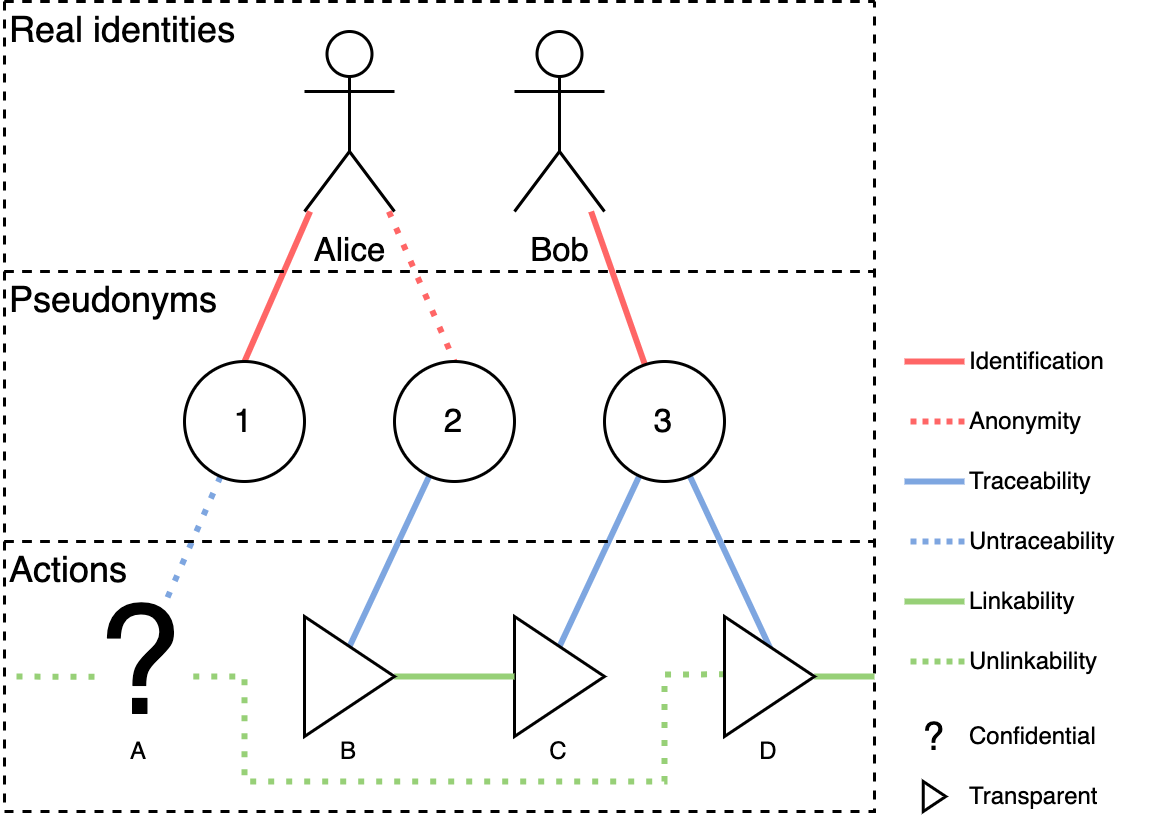
\includegraphics[width=9cm]{anonymity-diagram.png}
\centering
\caption{Let us assume Alice to be the customer willing to keep her identity anonymous and Bob to be the public SP. Alice controls two addresses, 1 and 2; the connection between her real identity and the first address has been compromised, and therefore the identification is possible; the connection between the second pseudonym is still unknown therefore anonymous. Alice takes two actions; the first one from the compromised address and the second one from the anonymous one. The first action is confidential; therefore, even though the pseudonym has been compromised, the action can not be associated with Alice. The second action is transparent; therefore, Alice maintain her anonymity as long as the connection to the second pseudonym is concealed.}

\label{fig:anonymity-diagram}
\end{figure}

The privacy-preserving blockchains are the ones that maintain anonymity via untraceability and (ideally) unlikability, not via the assumption that the connection between an address (pseudonym) and the real identity is concealed.   

Examples of blockchains that natively support confidential transactions are: Monero~\cite{vansaberhagenCryptoNote2013} (via Ring Signatures~\cite{noetherRingSignatureConfidential2015} and Bulletproofs~\cite{moneroBulletproofsMoneropediaMonero, bunzBulletproofsShortProofs2018}), ZCash~\cite{ben-sassonZerocashDecentralizedAnonymous2014} (via zkSNARK~\cite{ben-sassonSNARKsVerifyingProgram2013}), and Grin~\cite{fuchsbauerAggregateCashSystems2019} (via Mimblewimble~\cite{jedusorMIMBLEWIMBLE2016}).

Overly techniques that achieve anonymity on top of non-privacy-preserving blockchains are: Ethereum's Tornado Cash\cite{pertsevTornadoCashPrivacy2019} (via zkSNARK~\cite{grothSizePairingbasedNoninteractive2016} and MiMC~\cite{albrechtMiMCEfficientEncryption2016}), Bitcoin's Wasabi\footnote{https://wasabiwallet.io/} (via CoinJoin \cite{maxwellCoinJoinBitcoinPrivacy2013}).

\subsection{Payment for services}\label{payment-for-services}
Transactions between customers and SPs must be pegged to prevent proving one payment for multiple transactions. In other
words, we need a mechanism that uniquely associates a payment with the corresponding transaction.

Depending on a cryptocurrency, the link can be created in different
ways:
% continue reading from here
\begin{itemize}

\item separate address: each transaction derives a new address uniquely associated with the transaction. Such addresses can be derived using Hierarchical Deterministic Wallets (BIP-32)\footnote{https://github.com/bitcoin/bips/blob/master/bip-0032.mediawiki}.
\item memo: the payments are sent to one SP account but contain an extra field named ``memo'' filled with the unique number provided by the SP in $\mathrm{PoD}$. Each payment containing such value in the memo is considered to pay for the transaction. In case of a dispute, revealing both the payment memo and the $\mathrm{PoD}$ proves the connection.
\end{itemize}

Both approaches have some advantages and disadvantages, but our protocol can abstract them away by treating them as some randomly generated unique number, often called \textit{nonce} (number once). The actual implementation depends on a particular blockchain.

In case of a dispute, there must be a way to prove to the justice that the customer has paid for the transaction. As the proof of transaction is trivial in transparent and trackable blockchains, it gets more complicated when it comes to anonymous blockchains. Monero allows proving and checking payments via dedicated API \cite{MoneroHowProve}. ZCash provides a mechanism called Payment Disclosure \cite{daviesIntroductionPaymentDisclosure2017}.

\subsection{Storage network}\label{storage-network}
Once the SP finishes its service, he has to provide the result to the customer. The most natural approach would be to send the result via e-mail or some dedicated platform. However, since the customer wants to stay anonymous, he does not want to expose his e-mail address nor IP address. Moreover, the SP should prove that the result has been provided before the deadline, which brings us to the issue of proof of existence discussed in section ~\ref{sec:message-board}.

One approach would be to post the result into a blockchain. However, storing data on a blockchain is very expensive. The most common workaround (\cite{shahidBlockchainBasedAgriFoodSupply2020, wangAuditableProtocolsFair2019, chenImprovedP2PFile2017}) is to publish the data on a content addressable peer-to-peer storage network like IPFS~\cite{benetIPFSContentAddressed2014}. Then, publish on the blockchain just the content identifier ($\mathrm{cid}$) that uniquely points to the content stored on IPFS.

We take the same approach. Once the SP creates the result, he encrypts it using the previously provided encryption key and uploads it to the IPFS network.

To increase anonymity, the customer should use standard techniques to hide its IP address, such as gateway, VPN, proxy, or onion routing.

\subsection{Separation of concerns}
We could use one blockchain to achieve all of these three roles: (i) anonymous payments, (ii) message board, (iii) storage network.

While most blockchains could provide the message board functionality, anonymous payments are not as prevalent. Especially a provable storage network is a functionality of a few specialized blockchains.

Instead of searching for one blockchain that provides all the functionalities, we allow the protocol to use separate blockchains for each role. If a suitable blockchain arises, it can play more than one role.

At the time of writing, we see the following technologies that fulfil the requirements of each role:

\begin{enumerate}
\def\labelenumi{\arabic{enumi}.}

\item Anonymous payments: Monero \cite{vansaberhagenCryptoNote2013}, ZCash
  \cite{ben-sassonZerocashDecentralizedAnonymous2014}, Grin \cite{fuchsbauerAggregateCashSystems2019},
  Tornado Cash \cite{pertsevTornadoCashPrivacy2019}.
\item Message board: Stampery \cite{crespoStamperyBlockchainTimestamping2017}, Proof of Existence
  \cite{ProofExistenceOnline} (Bitcoin blockchain), Chainpoint
  \cite{ChainpointBlockchainProof} (Bitcoin blockchain), or any other blockchain that
  supports attaching extra data along the transaction.
\item Storage network: IPFS \cite{benetIPFSContentAddressed2014}, Filecoin
  \cite{protocollabsFilecoinDecentralizedStorage2017} (runs on top of IPFS), or Ethereum's
  Swarm\cite{teamSWARMStorageCommunication2021}.
\end{enumerate}

\section{The Protocol}\label{sec:protocol}

\subsection{Prerequisites}
We do not design our protocol with the assumption of using particular technologies; instead, we define requirements that each party must satisfy to make the whole system work together. The choice of the particular technology for each role is up to the developer.

\begin{itemize}
\item There exists common PKI infrastructure:
    \begin{itemize}
        \item The customer and the SP have their key pairs consisting of secret key $\mathrm{sk}(\mathrm{party})$ and public key $\mathrm{pk}(\mathrm{party})$, where $\mathrm{party} \in \{\mathrm{C}, \mathrm{SP}\}$ is the customer or the service provider accordingly.
        \item Both the customer and the SP can create and verify digital signatures created by the customer $\mathrm{sig}_{\mathrm{sk}(\mathrm{C})}$ and the SP $\mathrm{sig}_{\mathrm{sk}(\mathrm{SP})}$.
        \item The SP's public key $\mathrm{pk}(\mathrm{SP})$ is publicly known.
    \end{itemize}
    
\item Both the customer and the SP:
    \begin{itemize}
        \item use common symmetric encryption $\mathrm{E}_\mathrm{key}(\cdot)$ and decryption $\mathrm{D}_\mathrm{key}(\cdot)$ operations.
    \end{itemize}

\item The SP:
    \begin{itemize}
        \item accepts packages from unknown customers and give $\mathrm{PoD}$ in return.
        \item accepts payments with anonymous cryptocurrencies as described in section~\ref{payment-for-services}.
    \end{itemize}
    
\item Justice:
    \begin{itemize}
        \item accepts as evidence in a dispute the $\mathrm{PoD}$, $\mathrm{PoP}$, and payment $\mathrm{attestation}$ as described in section~\ref{fairness}.
    \end{itemize}

\item Anonymous payments:
    \begin{itemize}
        \item supports anonymous, i.e., untraceable and (ideally) unlinkable transactions as specified in section~\ref{sec:pseudo-anon}.
        \item supports uniquely identifying transaction either via separate address, memo field, or other similar mechanisms as described in section ~\ref{payment-for-services}. 
    \end{itemize}

\item Message board:
    \begin{itemize}
        \item supports proofs as large as the size of $\mathrm{PoP}$, i.e., sum size of $\mathrm{cid}$, $\mathrm{nonce}$, and $\mathrm{sig}$.
    \end{itemize}

\item The storage network:
    \begin{itemize}
        \item allows for uniquely content retrieval via $\mathrm{cid}$ (usually a hash of the content).
        \item allows for anonymous content retrieval.
    \end{itemize}
\end{itemize}

\subsection{Messages}\label{messages}
In this section, we describe the messages exchanged between the parties of the protocol.

\vspace{5mm}

\noindent \textbf
{Package}\label{package} is a physical container prepared by the customer encompassing all $\mathrm{materials}$ required by the SP to provide the service, and an encryption $\mathrm{key}$ used to encrypt the result published on the storage network.

$$\mathrm{pkg} \equiv (\mathrm{materials}, \mathrm{key})$$

where:

\begin{itemize}

\item $\mathrm{materials}$ - are the materials required to provide the service, for example, samples of urine, blood, stool, saliva; legal documents, CDs, emails, photos, bank statements; or any other kind of evidence depending on the service.
\item $\mathrm{key}$ - symmetric key used to encrypt and decrypt the result.
\end{itemize}

\noindent \textbf
{Proof of delivery ($\mathrm{PoD}$)}\label{proof-of-delivery} is a  confirmation issued by the SP to the customer that proves that the customer has delivered to the SP a complete (according to the SP requirements) package, and the SP accepted it.

It is also an agreement between the customer and the SP, as it includes agreed upfront deadlines of actions in the protocol.

We assume the $\mathrm{PoD}$ to be a QR code printed on a paper receipt, but any other form that guarantees integrity, authenticity, and non-repudiation can be used instead. 

$$\mathrm{PoD} \equiv (\mathrm{T}_\mathrm{issue}, \mathrm{T}_\mathrm{pay}, \mathrm{T}_\mathrm{provide}, \mathrm{nonce}, \mathrm{sig}_\mathrm{SP})$$

where:

\begin{itemize}

\item $\mathrm{T}_\mathrm{issue}$ - time at which the $\mathrm{PoD}$ is issued.
\item
  $\mathrm{T}_\mathrm{pay}$ - deadline to pay for the transaction.
\item
  $\mathrm{T}_\mathrm{provide}$ - deadline to provide a result of the service.
\item $\mathrm{nonce}$ - randomly generated number uniquely identifying the transaction.
\item $\mathrm{sig}_\mathrm{SP}$ - the SP's signature guaranteeing non-repudiation.
\end{itemize}

also:
\(\mathrm{T}_\mathrm{issue} < \mathrm{T}_\mathrm{pay} < \mathrm{T}_\mathrm{provide}\)

\noindent \textbf
{Proof of provision ($\mathrm{PoP}$)}\label{proof-of-provision} is proof that the SP published the result at a certain time. It defends the SP in case the customer unjustly starts a dispute after the result has been published. The connection between $\mathrm{PoP}$ and the result is made by the content identifier ($\mathrm{cid}$) that uniquely identify the result (it is some kind of a hash of the result) such that the result can not be forged after the $\mathrm{PoP}$ has been published.

The $\mathrm{PoP}$ is a digital construction published by the SP on the message board.

\[\mathrm{PoP} \equiv (\mathrm{cid}, \mathrm{nonce}, \mathrm{sig}_\mathrm{SP})\]

where:

\begin{itemize}

\item
  \(\mathrm{cid}\) - content identifier as specified in section~\ref{storage-network}.
\item
  \(\mathrm{nonce}\) - the value uniquely identifying the transaction previously generated in $\mathrm{PoD}$.
\item
  \(\mathrm{sig}_\mathrm{SP}\) - the SP's signature guaranteeing authentication.
\end{itemize}

\noindent \textbf
{Payment attestation}\label{payment-attestation} proves that the customer did the payment. Since the evidence depends on a particular blockchain (see section ~\ref{payment-for-services}), we refer to it symbolically as
\(\mathrm{attestation}\).

\noindent \textbf
{Result}\label{results} is assumed to be a document in PDF format, but any other format is allowed as long as it can be binary encoded and uploaded to IPFS. We refer to it symbolically as $\mathrm{result}$.

\noindent \textbf
{Content Identifier (cid)}\label{content-identifier-cid} is a term coined by IPFS\footnote{https://docs.ipfs.tech/concepts/content-addressing}. However, since our protocol does not depend on
this particular implementation of the storage network, we let the $\mathrm{cid}$ be any other identifier that securely and uniquely points to the content.

\subsection{Protocol description}\label{protocol-description}

In this section, we describe each step of the protocol, also shown in the figure~\ref{fig:protocol-diagram}.

\begin{figure}[h!]
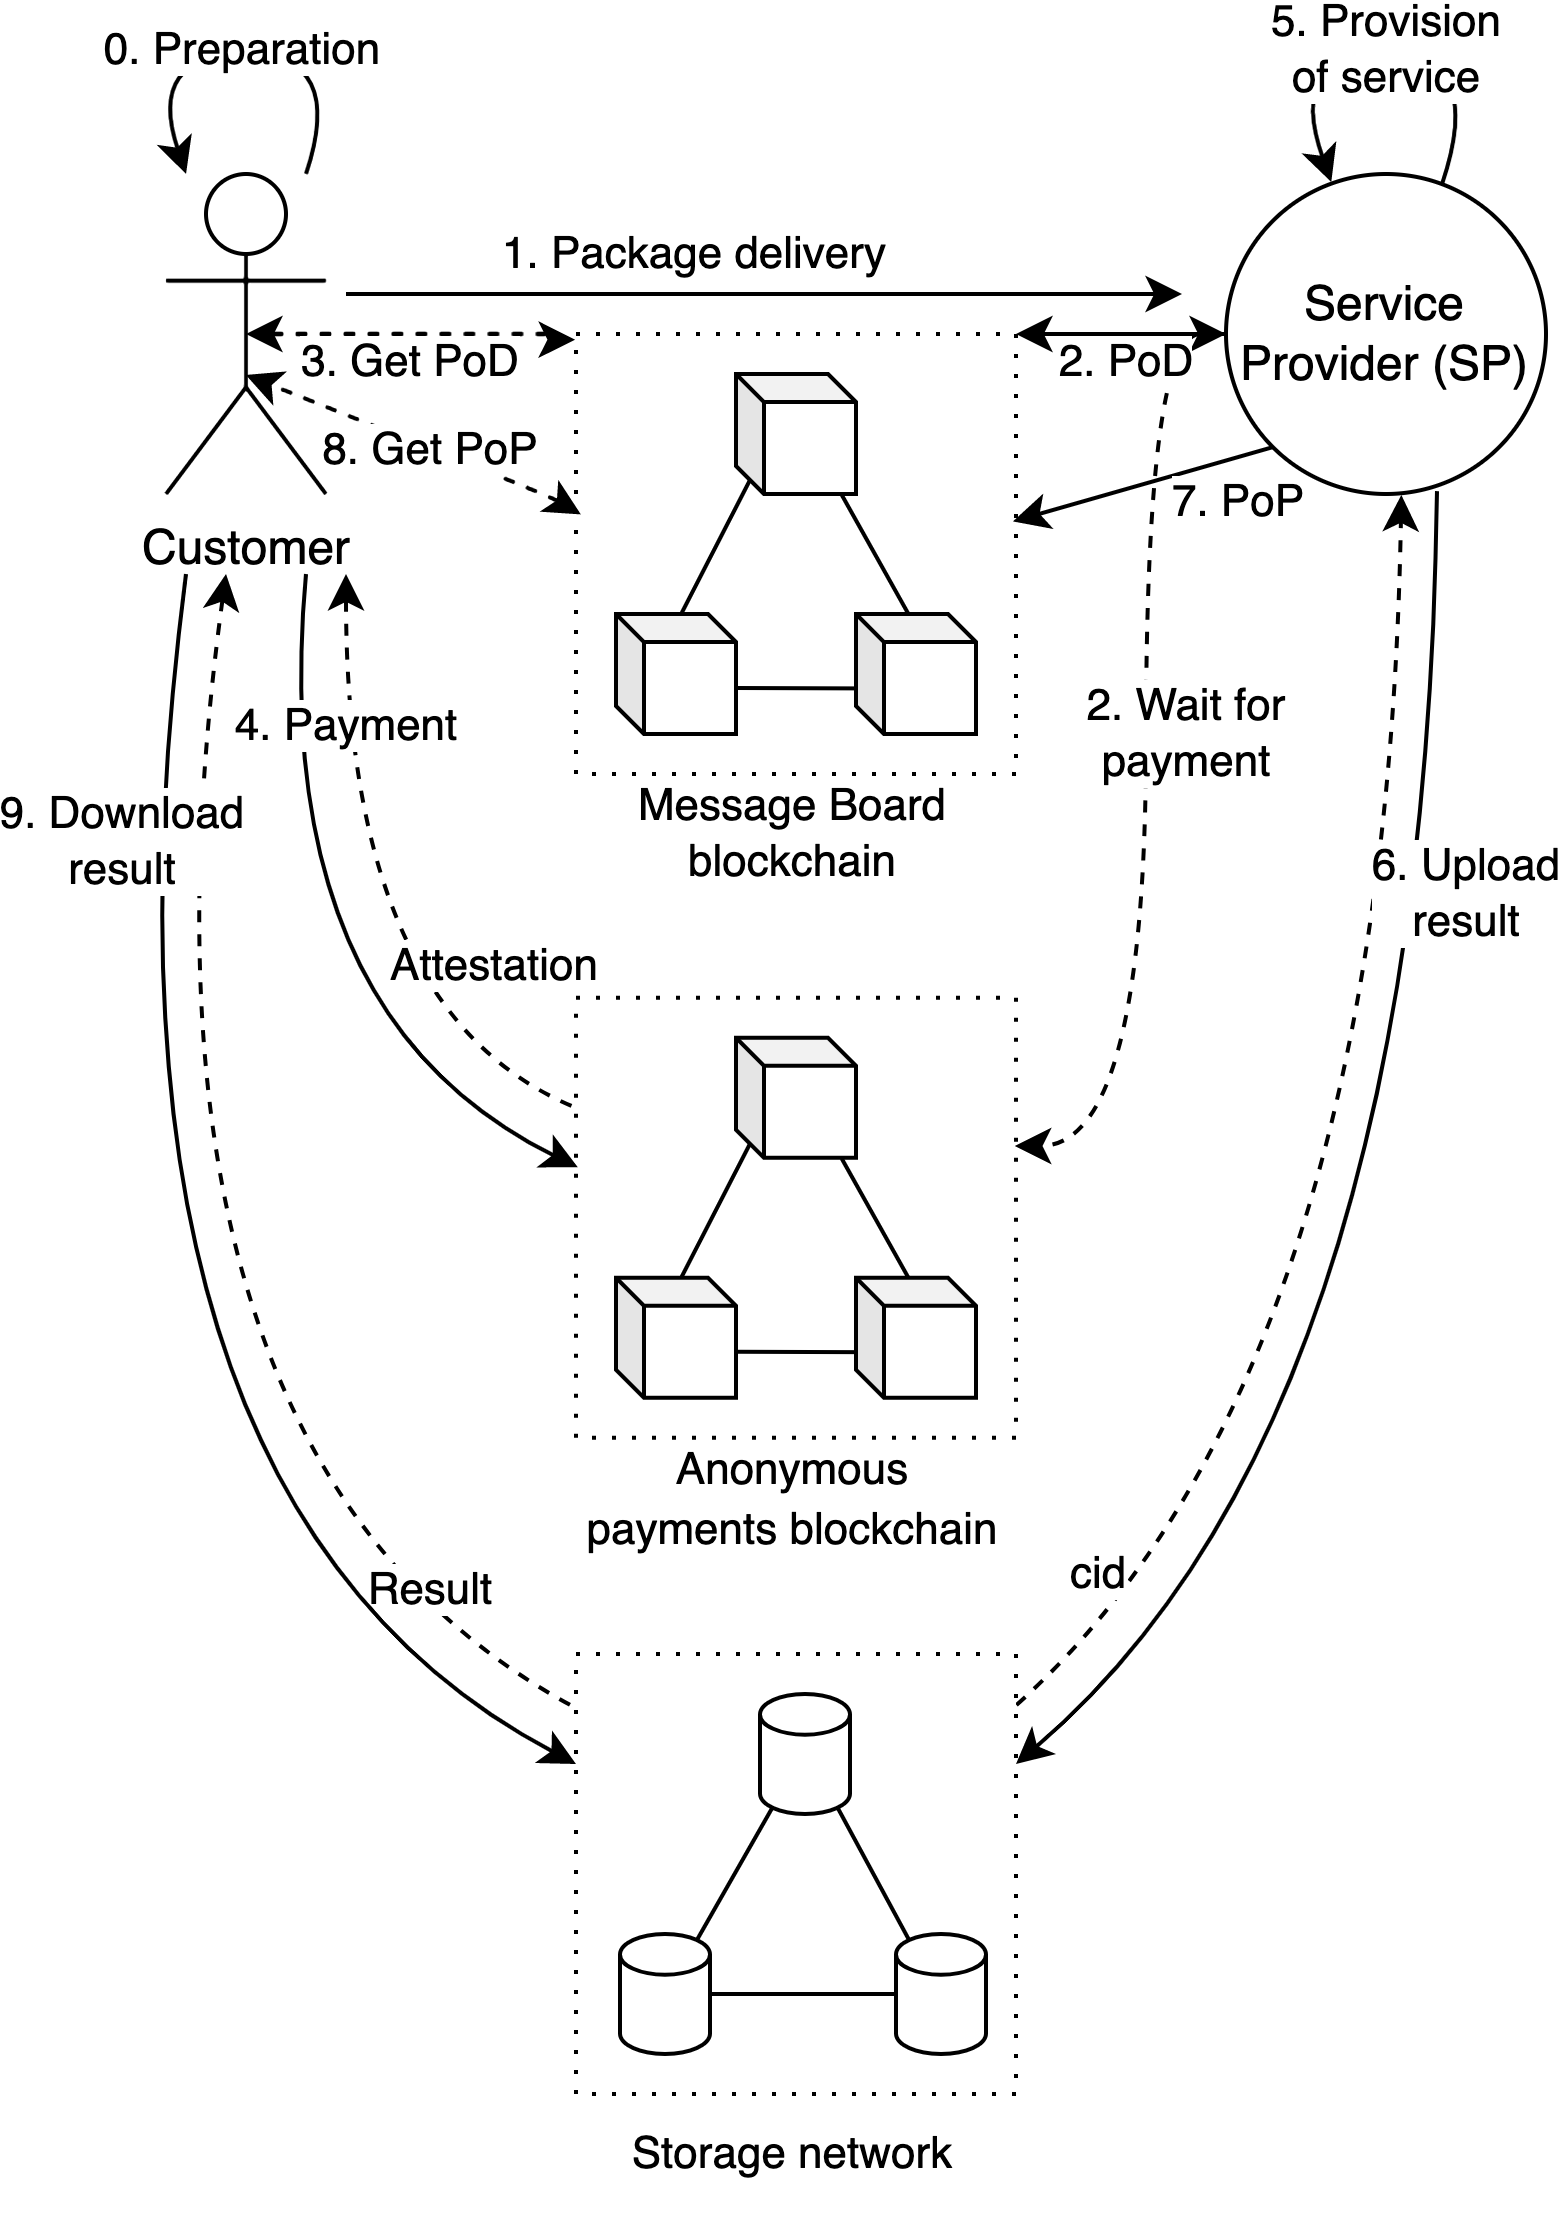
\includegraphics[width=\linewidth]{anonser-protocol.png}
\centering
\caption{Messages exchanged in the protocol.}
\label{fig:protocol-diagram}
\end{figure}

\noindent \textbf
{Step 0.  Preparation}\label{step-0-preparation}

The customer collects all the $\mathrm{materials}$ required by the SP, generates an encryption $\mathrm{key}$, prints it on a paper as a QR code, and packs them together into a package $\mathrm{pkg}$.

Symbolically: 
\[
\mathrm{pkg} \gets (\mathrm{materials}, \mathrm{key})
\]

\noindent \textbf
{Step 1. Package delivery}\label{step-1-package-delivery}

They protocol starts once the customer delivers package $\mathrm{pkg}$ and the SP accepts its content. In return, the SP issue a $\mathrm{PoD}$ with agreed upfront payment deadline $\mathrm{T}_\mathrm{pay}$, service provision deadline $\mathrm{T}_\mathrm{provide}$, and current time $\mathrm{T}_\mathrm{issue}$. Also, the $\mathrm{PoD}$ consist of randomly generated unique number $\mathrm{nonce}$, which will allow associating all actions related to the transaction throughout the protocol. Finally, the digital signature $\mathrm{sig}_{\mathrm{sk}(\mathrm{SP})}$ on the $\mathrm{PoD}$ created with the SP's secret key $\mathrm{sk}(\mathrm{SP})$ guarantee non-repudiation.

We assume this step to be entirely physical, i.e., $\mathrm{pkg}$ consists of physical materials, $\mathrm{PoD}$ is in the form of, e.g., QR code printed on a paper receipt. 

$\mathrm{PoD}$ could be published on a message board (similarly to $\mathrm{PoP}$); however, since the $\mathrm{pkg}$ is delivered personally or via a trusted person, the confirmation can be issued in person. If we would like to hire a courier to deliver our $\mathrm{pkg}$, then the $\mathrm{PoD}$ would have to be published on the message board (further extension to the anonymous delivery system is discussed in section \ref{sec:future-work}).

Symbolically: 
\[
\mathrm{PoD} \gets \mathrm{delivery}(\mathrm{pkg})
\]
\[
(\mathrm{T}_\mathrm{issue}, \mathrm{T}_\mathrm{pay}, \mathrm{T}_\mathrm{provide}, \mathrm{nonce}, \mathrm{sig}_{\mathrm{sk}(\mathrm{SP})}) \equiv \mathrm{PoD}
\]

\noindent \textbf
{Step 2. Payment}\label{step-2-payment}

Having the $\mathrm{PoD}$ issued, the SP can not reject receiving the package. At this point the
customer should pay for the transaction (identified by $\mathrm{nonce}$ value) with the agreed upfront cryptocurrency blockchain (see section~\ref{payment-for-services}).

In return, the customer receives the $\mathrm{attestation}$ that should be disclosed in case of a dispute.

Symbolically: 
\[
\mathrm{attestation} \gets \mathrm{payment}(\mathrm{nonce}, \mathrm{sig}_{\mathrm{sk}(\mathrm{C})})
\]

\noindent \textbf
{Step 3. Provision of service}\label{step-3-provision-of-service} 
Once the customer has paid for the transaction, the SP starts providing the service.

Symbolically: 
\[
\mathrm{result} \gets \mathrm{provision}(\mathrm{materials})
\]

\noindent \textbf
{Step 4. Upload result }\label{step-4-results-upload}

After the service is finished, a result should be created. Next, the result is encrypted using encryption symmetric $\mathrm{key}$ provided in the first step.

The encrypted result is then uploaded on the content addressable network such as IPFS. In return the content identifier ($\mathrm{cid}$) is created.

Symbolically: 
\[
\mathrm{cid} \gets \mathrm{upload}(E_{\mathrm{key}}(\mathrm{result}))
\]

\noindent \textbf
{Step 5. Proof of provision}\label{step-5-proof-of-provision-publication}

When the result is published, the SP performs proof of provision by publishing $\mathrm{cid}$ along with $\mathrm{nonce}$ and signature $\mathrm{sig}_\mathrm{SP}$.

Symbolically: 
\[
\mathrm{PoP} \equiv (\mathrm{cid}, \mathrm{nonce}, \mathrm{sig}_{\mathrm{sk}(\mathrm{SP})})
\]
\[
\mathrm{publish}(\mathrm{PoP})
\]

\noindent \textbf
{Step 6. Pull proof of provision}\label{step-6-proof-of-provision-notification}

After delivering the package and paying for the transaction, the customer subscribes to the message board and waits until the SP publishes the proof of provision. The subscription is for the SP public key $\mathrm{pk}(\mathrm{SP})$ and transaction's $\mathrm{nonce}$.

Symbolically: 
\[
\mathrm{cid} \gets \mathrm{subscribe}(\mathrm{pk}(\mathrm{SP}), \mathrm{nonce})
\]

\noindent \textbf
{Step 7. Result download}\label{step-7-results-download} 
Having the $\mathrm{cid}$, the customer downloads and decrypts the $\mathrm{result}$.

Symbolically: 
\[
\mathrm{result} \gets \mathrm{D}_{\mathrm{key}}(\mathrm{download}(\mathrm{cid}))
\]

\section{Experiments}\label{sec:experiments}

\subsection*{Setup}

We have developed a prototype of our protocol using the following technologies:

\begin{itemize}
  \item{Anonymous payments} — we use the Monero blockchain \cite{noetherRingSignatureConfidential2015}.
  \item{Storage netowork} — we use the Powergate\footnote{https://github.com/textileio/powergate}, which is a wrapper around Filecoin and IPFS.
  \item{Message board} — we use the Ethereum blockchain \cite{woodEthereumSecureDecentralised2014}; concretely, Truffle Ganache\footnote{https://trufflesuite.com/ganache/} and Solidity language.
  \item{Customer and SP} — we create client-side web application (webapp) using React for UI, web3.js for interaction with Ethereum, and crypto-js for encryption. We use MetaMask browser extension for signing and submiting transactions to Ethereum's node. We use `monerod` and `monero-wallet-cli' command-line tools for interacting with Monero blockchain.
\end{itemize}

The prototype is available at \url{https://anonser.stan.bar}. The source code is available at \url{https://github.com/stanbar/anonymous-provision-of-services-via-blockchain}.

We developed and tested our prototype in the following environment:

\begin{itemize}
  \item{OS} — Arch Linux 5.11.8
  \item{Docker} — 20.10.5
  \item{CPU} — Intel(R) Core(TM) i7-4790 (8) 4.00~GHz
  \item{RAM} — 16 GB DDR3
  \item{Storage} — Samsung PM85 256~GB SSD

  \item{monerod and monero-wallet-cli} — v0.18.1.2-release
  \item{Powergate} — v0.1.6 // get the version from `docker ps`
  \item{Ganache} — v7.5.0
  \item{Solidity} — v0.8.17
  \item{ReactJS} — v18.0.25
  \item{web3.js} — v1.8.1
  \item{crypto-js} — v4.1.1
\end{itemize}

For simplicity, all components run on one, mentioned above, physical machine; and all processes are managed by Docker. 

Moreover, Powergate is configured to use local Filecoin and IPFS networks.
For Ethereum blockchain we use Truffle Ganache, which is a local Ethereum blockchain for development and testing purposes. 
Monero is configured to use the public stage network.

\subsection*{Experiments}

\paragraph{Preparation}

Both customer and SP create a Monero wallets using `monero-wallet-cli' command-line tool.

Service provider deploys the smart contract using the `truffle migrate --network development` command, which deploys the smart contract to the local Ethereum blockchain. The webapp is configured to use the latest deployed smart contract address.

Customer get some testing funds using \url{https://community.rino.io/faucet/stagenet/} faucet service.

Next, the customer enable per-transaction proof generation by setting `set store-tx-info 1` for his wallet.  The proof generation is required to verify the payment in case of dispute.

At this point both the customer and the SP are ready to start the protocol.

\paragraph{Experiment}

Service Provider (SP) and Customer (C) are two different users of our prototype, but for simplicity they use the same machine and the same web application.

Now we describe the experiments we performed to test our protocol.

\begin{itemize}
  \item 1. The protocol starts with the Customer opening the webapp and creating new provision. 
The app generates random ECDSA (secp256k1) client's keypair and random 32 bytes provisionID, then display QR code that encodes both the provisionID and the client's public key. 
The private key must be stored and provided later for the decryption of the results.

  \item 2. The Customer prints the QR code and put it on a package.

  \item 3. The Customer delivers his package to the SP either: in person, via trusted party, or delivery agency.

  \item 4. The SP opens the app, scans the QR code decoding the provisionID and the client's public key.

  \item 5. Since (in this experiment) the provision has not been paid in cash, the SP submits a Proof of Delivery transaction to the Ethereum blockchain, indicating that fact setting the `paid` flag to `false`, and `paymentAddress` field with dedicated Monero address using `monero-wallet-cli integrated-address`.
 If the provision is paid with cash, the SP proceed to the step 8. Otherwise, the SP waits until the Customer pays for the provision.

  \item 6. The Customer (using the webapp) check the transaction status on the Ethereum blockchain invoking `getProvision(clientPubKey, provisionID)`.

  \item 7. The Customer (using the `monero-wallet-cli transfer`) sends the payment to the designated in the smart contract `paymentAddress` and stores the .

  \item 8. The SP starts providing the service and outputs the file `result.pdf`.

  \item 9. The SP uploads the file `result.pdf` on the Filecoin and IPFS networks using Powergate. In result, SP gets the content identifier (`cid`), and `dealID`.

  \item 10. The SP submits a Proof of Provision transaction to the Ethereum blockchain by invoking `proofOfProvision(clientPubKey, provisionID, cid, dealID)`.

  \item 11. Meantime, the Customer subscribes to the Ethereum and waits until the SP publishes the Proof Of Provision.
 Once the Proof Of Provision is published the Customer downloads the result using either: IPFS network via https://dweb.link/<cid> or Lotus network using `lotus retreive <cid> <minerID>'. Then the results are decrypted using previously stored client's private key.

\end{itemize}

\section{Fairness analysis}\label{sec:fairness-analysis}

We analyze the fairness of the protocol by representing it as an interactive non-cooperative game.

\subsection{Model}\label{model}
We consider three positions:

\begin{itemize}
\item Neutral position (•): when a party has not spent nor gained anything of significant value (money, time, effort). For example, at the beginning of the protocol.
\item Disadvantaged position (-): when a party has put a significant value without receiving an equivalent. For example, the customer has paid for a service in advance.
\item Advantaged position (+): when a party would benefit if the transaction would halt at that step. For example, the SP has received payment before service provision.
\end{itemize}

There are many actions that each party can take, but we group them into two categories:

\begin{enumerate}
\def\labelenumi{\arabic{enumi}.}

\item Normal: taking actions prescribed by the protocol.
\item Abnormal: everything that deviates from the designed steps of the protocol. For example, sending an arbitrary message, skipping or repeating steps, timing out.
\end{enumerate}

Moreover, at any step of the protocol, the customer can start a dispute; therefore, another dimension with two positions has to be considered:

\begin{enumerate}
\def\labelenumi{\arabic{enumi}.}

\item Agree: the customer agrees with the action and therefore does not start a dispute.
\item Start a dispute: the customer disagrees with the action and therefore starts a dispute.
\end{enumerate}

As a result, in our analysis, we have to consider four different outcomes for each party of the protocol ($\mathrm{party \in \{c, s}\}$), for each step of the protocol ($\mathrm{step \in 1..7}$):

\begin{itemize}

\item
  $\mathrm{\sigma_{step,party,n}}$: after following the protocol when the other party acted normally.
\item
  $\mathrm{\sigma_{step,party,d}}$: after a settled dispute when the other party acted normally.
\item
  $\mathrm{\sigma_{step,party,\overline{n}}}$: after not starting a dispute despite the other party has acted abnormally.
\item
  $\mathrm{\sigma_{step,party,\overline{d}}}$: after a settled dispute when the other party has acted abnormally.
\end{itemize}



The protocol terminates after the last step, after starting a dispute, or after a party has not completed its designated action in time. Therefore, all positions except $\mathrm{\sigma_n}$ are termination positions.

Because the customer is anonymous, the SP can not start a dispute—there is no means to identify the customer. To mitigate the issue, we designed the protocol so that the SP who follows the protocol is always in an advantaged position, and therefore he has no reason to start a dispute. On the other hand, the customer can start a dispute at any time of the protocol, but only the actual misbehaviour of the SP makes him win the case.

\begin{definition}[Fairness] \label{def:fairness}
A protocol achieve fariness iff 
\begin{equation*}
\begin{split}
\forall_{party \in parties}\forall_{\mathrm{step} \in \mathrm{steps}} &\operatorname{can\ move}\\
&\operatorname{to\ the\ non-disadvantaged\ position} 
\end{split}
\end{equation*}

\end{definition}


\subsection{Assumptions}\label{assumptions}

Below  we listed assumptions we took for the analysis purpose.  

\begin{itemize}

\item
    Both parties start from a neutral position (•).
\item
    After completing a transaction, both parties end up in advantaged positions (+). In other words, they have intrinsic motivation to initialize and complete the transaction.
\item
    The protocol steps are atomic—there are no intermediate steps.
\item 
    The protocol can go only forward—there is no way of reverting any action.
\item
    Repeating the first step starts a new transaction. Repeating any other step is considered abnormal and gets ignored. For example, paying for the invoice twice does not cause any effect on the curse of the protocol.
\item 
    Once published, the result is available to the customer on the storage network. The idea of guaranteeing it cryptographically is discussed in section~\ref{sec:future-work}.
    
\item
    Winning the dispute leads to a neutral position (•).

\item
    Losing the dispute leads to a punishment greater than any reward, leading to a disadvantaged position (-). Hence, the rational customer will not start a dispute that he is unsure of winning.
\item
    Both the customer and the SP are rational (selfish). They always prefer to go from the worst position to a better position, but also risk a temporary worst position in favour of a later better position if and only if it is assured that they will not be stuck in the worst position.
\end{itemize}

\subsection{Steps}\label{steps}

Figure~\ref{fig:positions} shows the positions of each party after each possible action taken.

\begin{figure}[h!]
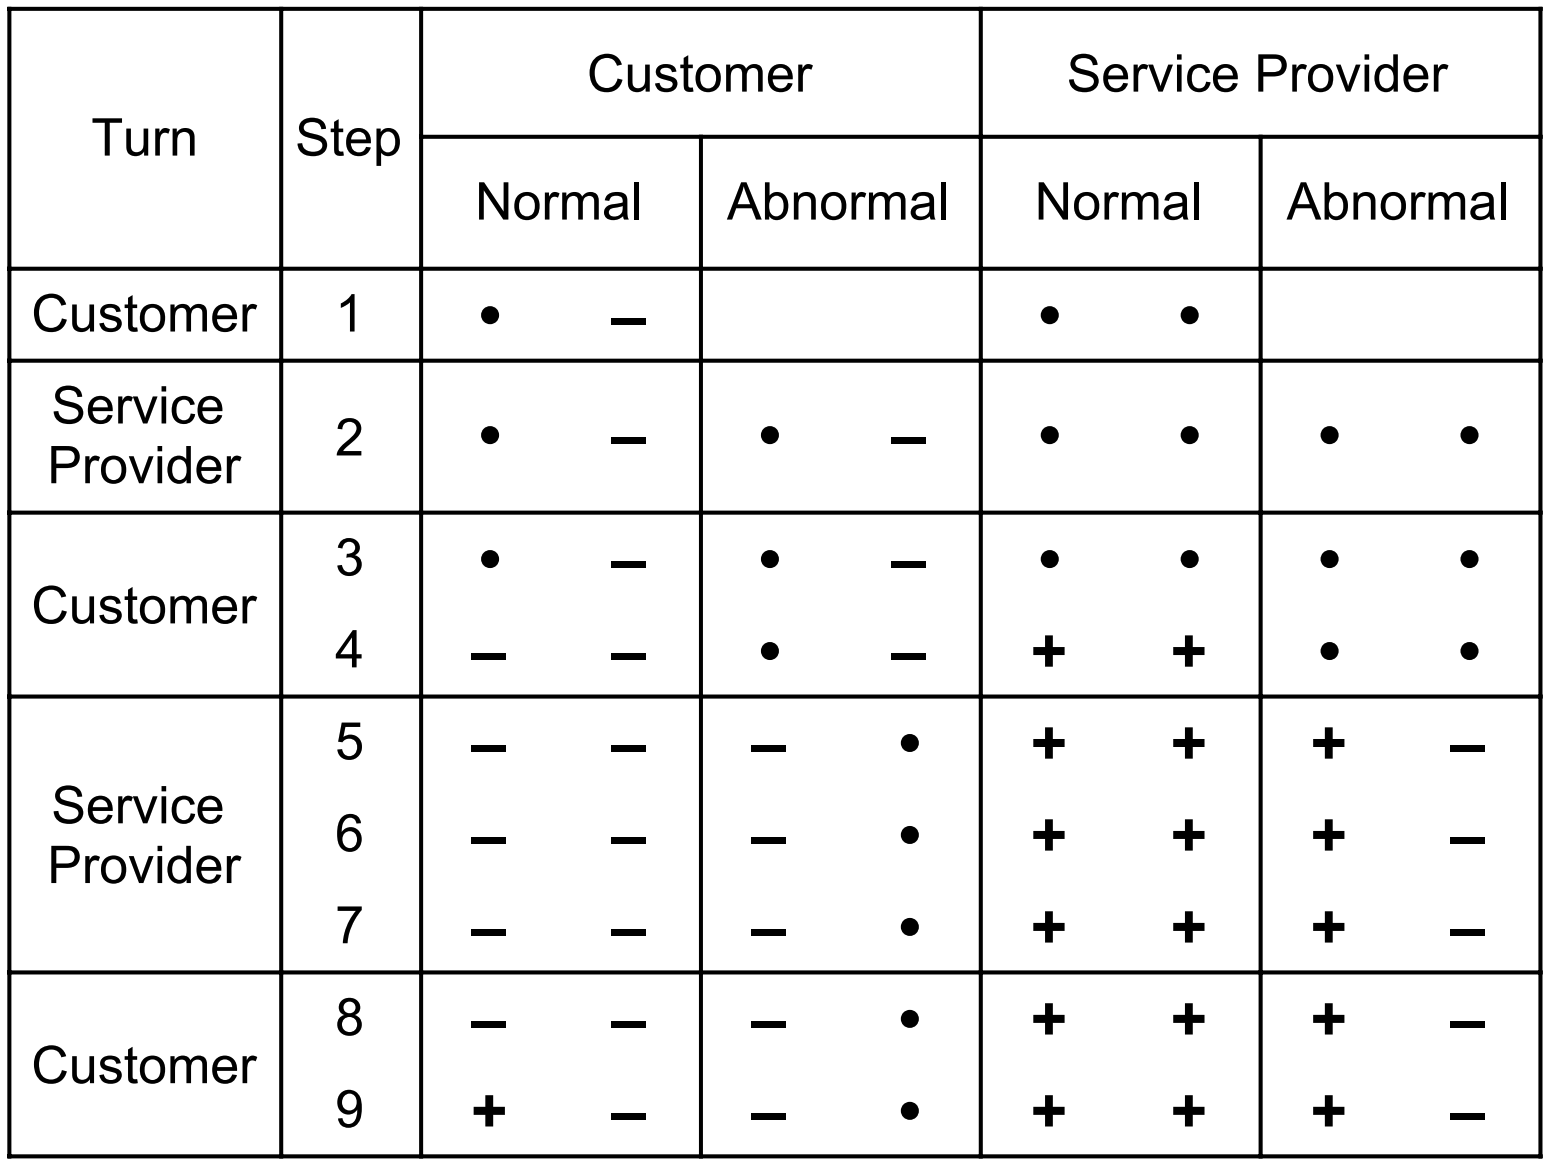
\includegraphics[width=9cm]{formal-table-of-positions.png}
\centering
\caption{Positions after each step of protocol}
\label{fig:positions}
\end{figure}

The description of each step and the rationale of the outcome position is given in the appendix in section \ref{sec:proof-of-fairness}.

\subsection{Example scenarios}\label{example-scenarios}

The figure~\ref{fig:misbehaviour} shows the transitions of positions when the SP tries to misbehave and does not execute service after receiving the payment. The customer reacts by starting a dispute and the protocol ends up neutral to the customer and disadvantaged to the SP positions.

\begin{figure}[h!]
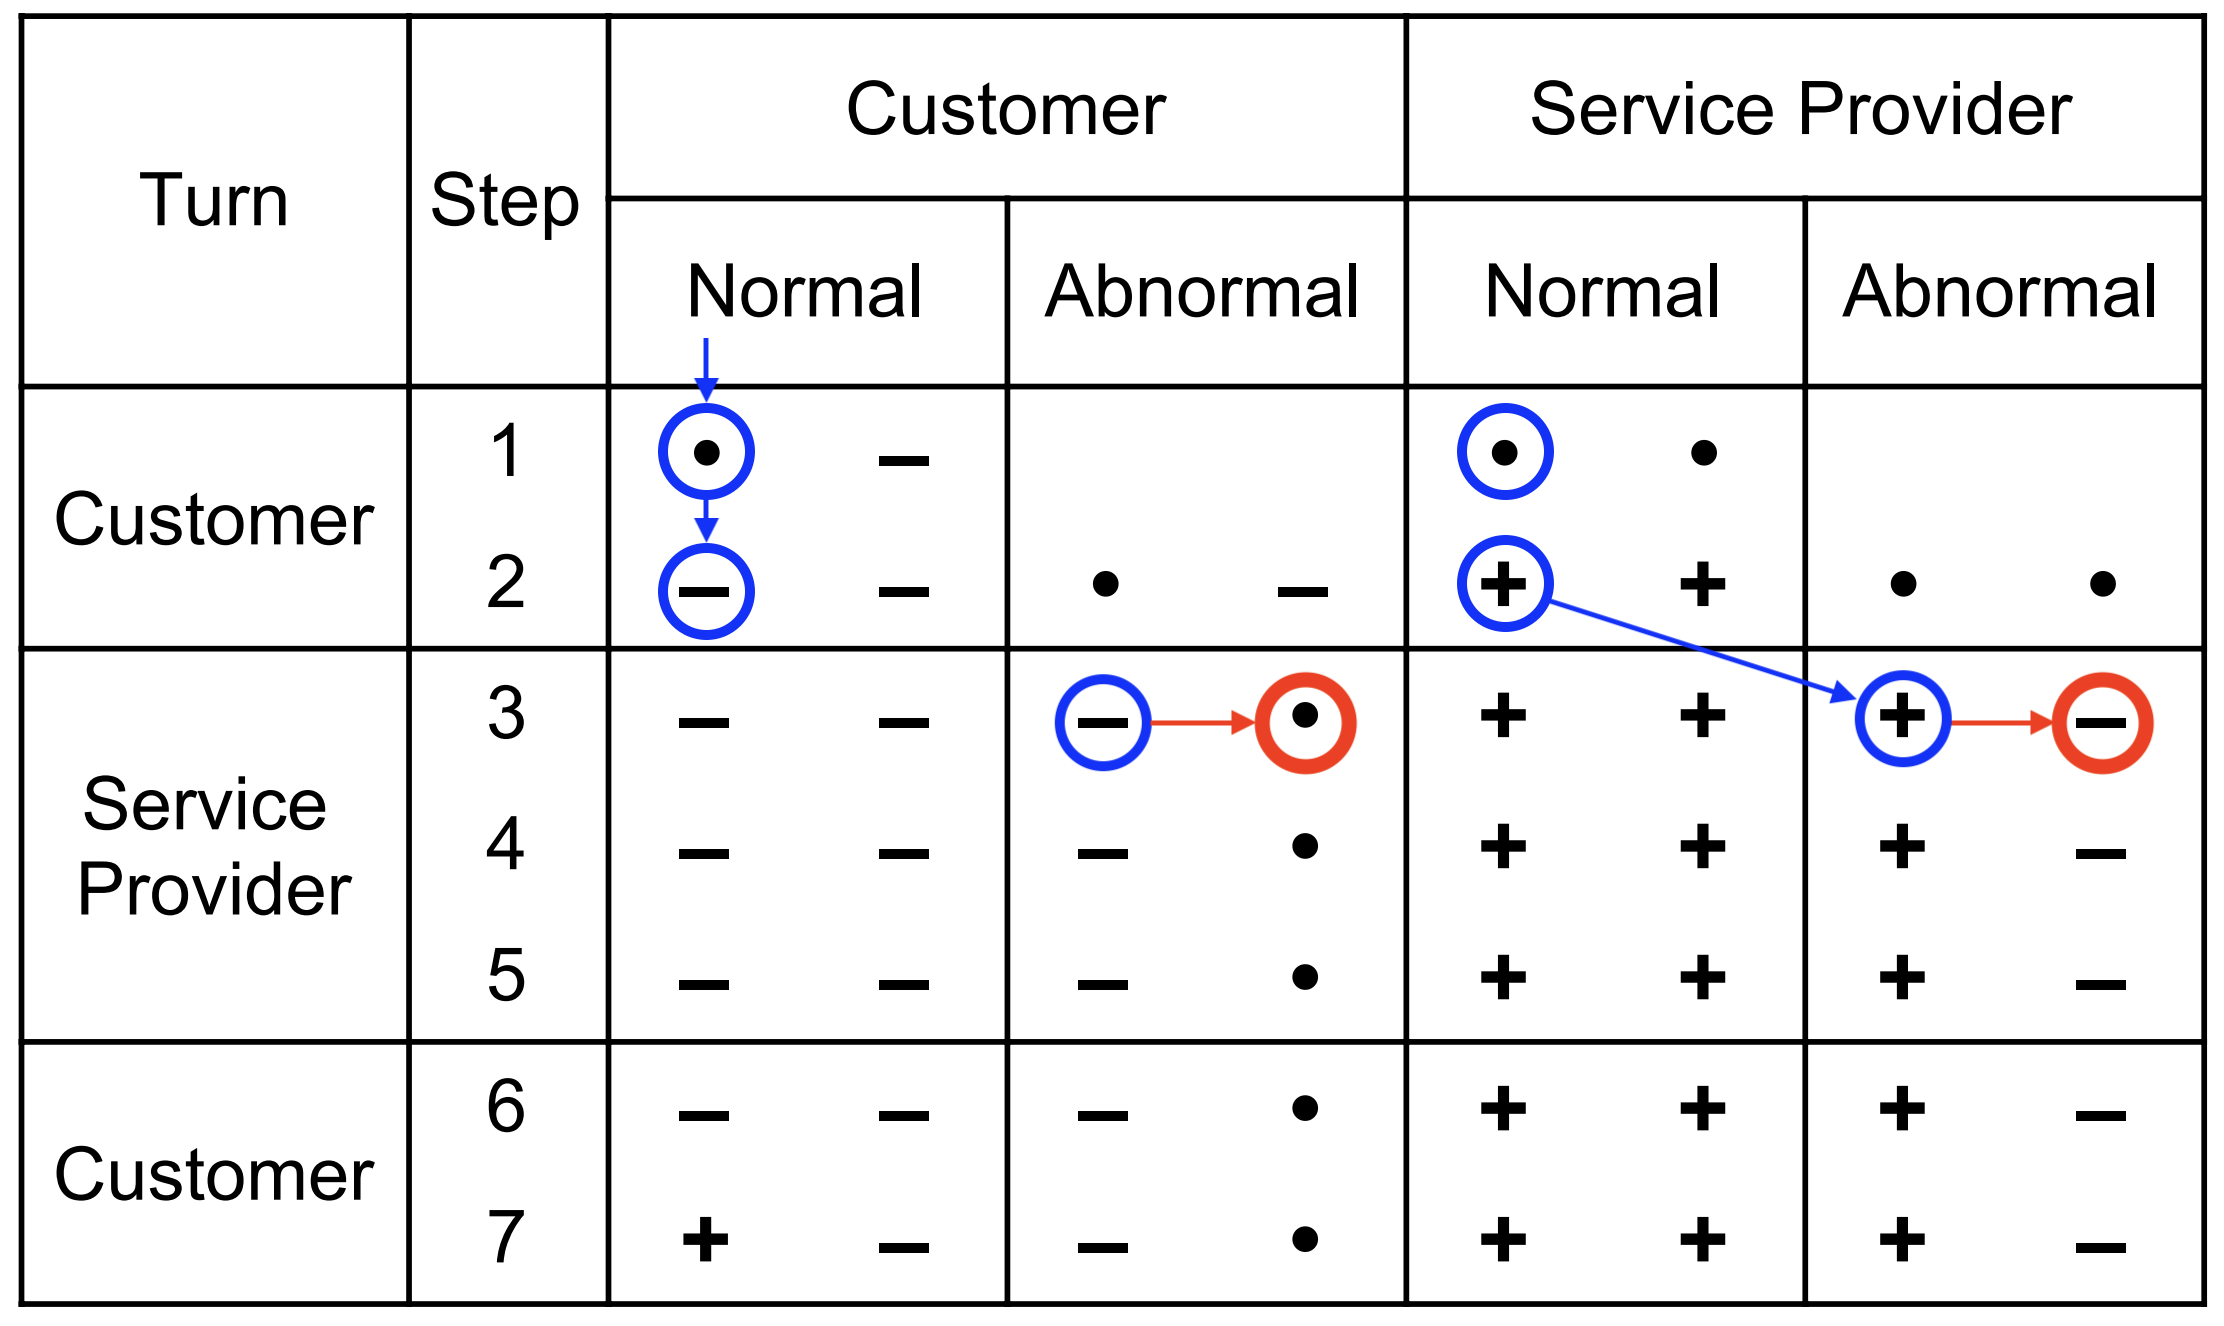
\includegraphics[width=9cm]{formal-misbehaviour-path.png}
\centering
\caption{Transitions of positions where the SP is misbehaving and the customer starts a dispute}
\label{fig:misbehaviour}
\end{figure}

Ultimately, the rational path for both parties is to follow the protocol as shown in the figure~\ref{fig:rational}.

\begin{figure}[h!]
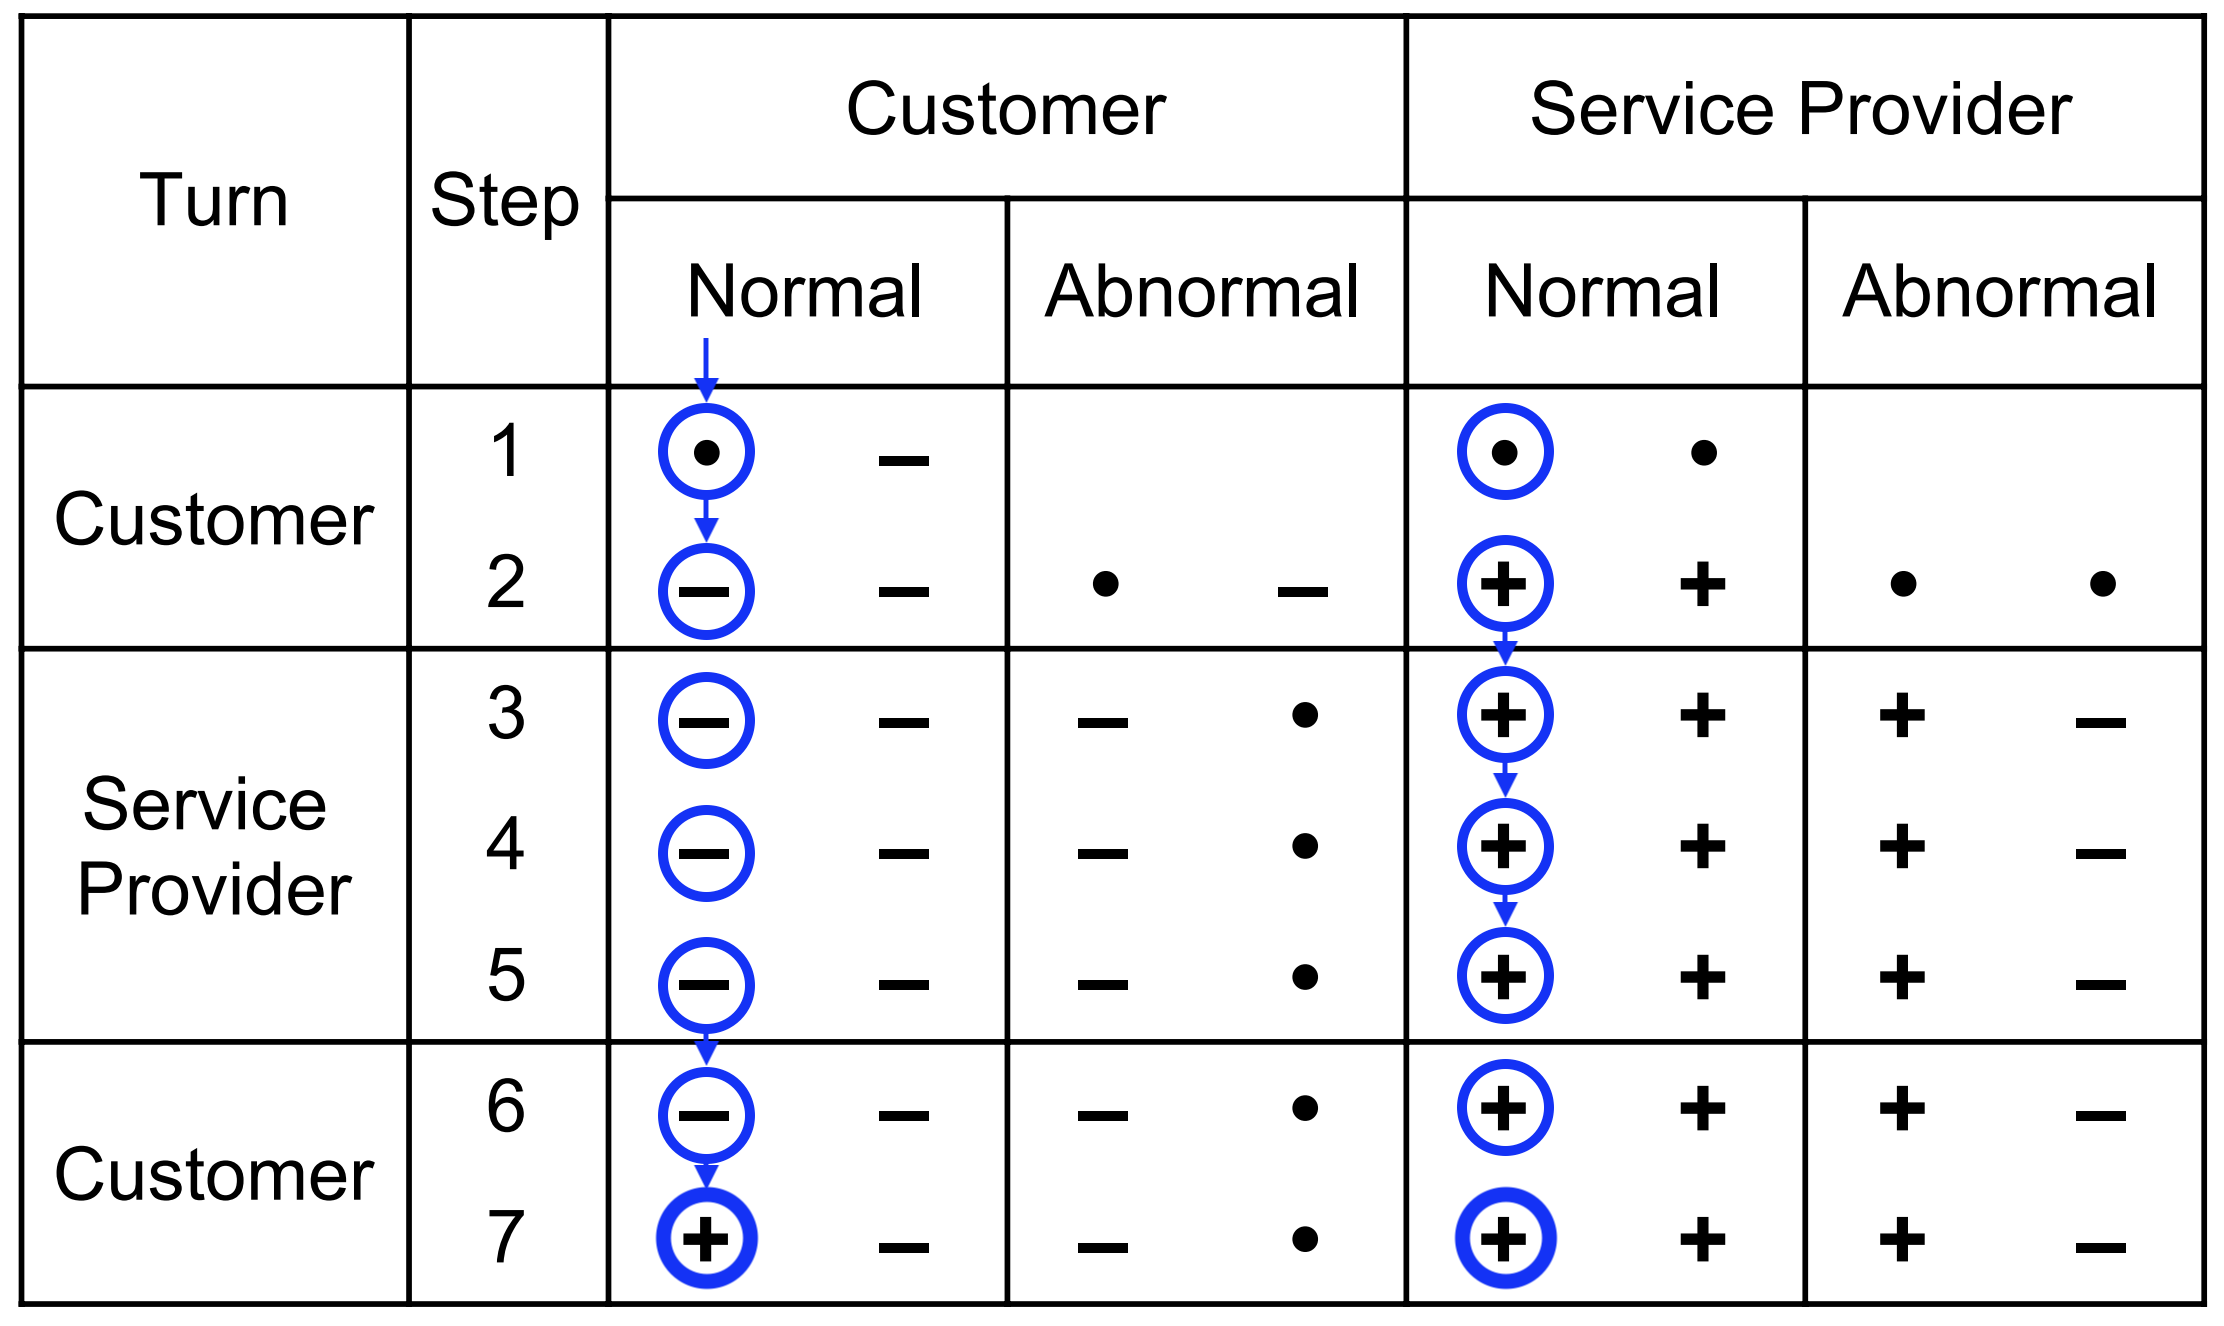
\includegraphics[width=9cm]{formal-rational-path.png}
\centering
\caption{Transitions of positions where where both the customer and the SP are behaving correctly}
\label{fig:rational}
\end{figure}

Using the fariness definition~\ref{def:fairness} and the assumptions stated in section~\ref{assumptions}, our analysis indicates that the protocol achieves fairness.


\section{Future work}
\label{sec:future-work}

\subsection{Justice}\label{justice}

Justice is the biggest obstacle in achieving a system that complies with Web 3.0 postulates\footnote{https://en.wikipedia.org/wiki/Web3}.

The possible directions for mitigation of such issues are to either (i) replace justice with decentralized autonomous organizations (DAO) like proposed in Themis~\cite{mengThemisDecentralizedEscrow2019} or Kleros~\cite{bergollaKlerosSociolegalCase2022}; or (ii) make it infeasible to provide incorrect results.

The first approach is more feasible in the near future. It would require creating a large set of experts in a field that, in case of dispute, would receive all the proofs ($\mathrm{PoD}$, $\mathrm{PoP}$, as well as any other proofs significant to the case) that could be queried by the experts in zero-knowledge fashion, i.e., they could ask a limited number of questions to the proofs and getting yes/no answers. The case would be fully confidential as they would not be able to query personal information. The experts would be incentivized to participate in the pool by the system of fees. They would be incentivized to vote honesty by the stake they would have to lock and reward/punishment they would get by judging correctly/incorrectly, where the ``correctly'' is determined by the quorum of votes.

The second approach is more philosophical and visionary. Suppose that the service we are undertaking is fully computable. Then, it would be possible by employing proofs of correctness of computations~\cite{ben-sassonSNARKsVerifyingProgram2013} to enforce that only correct computations (hence correct services) are accepted. It would require the complete service examination to be computable, which is hard to achieve in settings where physical materials (like blood) are examined. Concretely, the problem canes down to ``How to represent blood digitally?''. If we could represent urine, blood, saliva, or any other physical material in a binary format and let the customer take a sample, discrete it, and send it to the SP by himself, then the whole chain of integrity could be ensured. Therefore, wrong service provision would be infeasible.


\subsection{Provable availability of the
result}\label{cryptographically-provable-availability-of-results}

Currently, the SP has to publish the result into a peer-to-peer content-addressable storage network, e.g., IPFS. The problem is that nothing prevents the SP from publishing the result, receiving the $\mathrm{cid}$, publishing $\mathrm{PoP}$, and immediately after removing the result from the local storage. In case of dispute, the SP can upload the content again, proving its availability. The SP has no motivation to proceed with this kind of misbehaviour other than putting the customer in a disadvantaged position caused by the lost dispute. We see possible prevention of this misbehaviour by the usage of Filecoin—an incentive layer on top of IPFS that guarantees the content availability via economic incentivisations~\cite{protocollabsFilecoinDecentralizedStorage2017}. With the help of Filecoin, the SP would be obligated to create a deal that guarantees the availability of the result until the deadline of the transaction. Moreover, since Filecoin is a blockchain by itself, it could play both roles of message board and storage network.

\subsection{Paying with cash}\label{paying-with-cash}

Without loss of generality, the payment can be made with cash. The customer can exchange the cash with SP together with delivering the package. The $\mathrm{PoD}$ would contain information that the transaction has been paid with cash; therefore, steps one and two could be merged and realized in one step. In case of dispute, the payment disclosure would be included in $\mathrm{PoD}$.

\subsection{Anonymous delivery}\label{anonymous-delivery}

We assumed the customer to deliver the package to the SP personally or via a trusted person. However, the system could be extended to support an anonymous delivery system as proposed in Lelantos~\cite{altawyLelantosBlockchainBasedAnonymous2017}. One modification to the protocol would be to publish $\mathrm{PoD}$ on the message board, similarly to $\mathrm{PoP}$.

\section{Conclusions}\label{sec:conclusion}
In this paper, we have proposed the protocol for service provision that simultaneously achieves anonymity, fairness, dispute resolution, TTP-less, and support physical materials. The protocol can be employed to provide services without collecting any personal information. Payments are handled by anonymous cryptocurrencies. The result of the service is published on a content-addressable p2p network like IPFS. The dispute can be settled by disclosing the collected proofs to justice. 
Using the definition~\ref{def:fairness} we showed that the protocol achieves fairness by the proof of delivery, payment attestation, and proof of provision published on the message board blockchain. Finally, we pinpointed further improvements like decentralized dispute resolution, provable availability of the result, paying with cash, and anonymous package delivery via courier.

\bibliographystyle{IEEEtran}
% argument is your BibTeX string definitions and bibliography database(s)
\bibliography{bibliography}
\EOD


\begin{IEEEbiography}[{
\includegraphics[width=1in,height=1.25in,clip,keepaspectratio]{stanislaw.jpg}}]{Stanis\l{}aw Bara{\'n}ski} received BEng in 2019 and MSc in 2020 in informatics at Gdańsk University of Technology. 
Currently, he is a PhD candidate at the Department of Computer Architecture, Faculty of Electronics, Telecommunications and Informatics, Gdansk University of Technology.

His research interests include blockchains and cryptography, especially the issue of blockchain-based internet voting and mitigation of content poisoning attacks via blockchain.

He likes to develop his ideas right up to the commercialization stage. He is the author of multiple mobile and web applications that have reached success on the market. His blockchain-based internet voting project has been funded by the Stellar Community Fund for the most useful Stellar application. 
\end{IEEEbiography}

\begin{IEEEbiography}[{\includegraphics[width=1in,height=1.25in,clip,keepaspectratio]{julina.jpg}}]{JULIAN SZYMA{\'N}SKI}  received the PhD degree in 2009 and DSc in 2020 at Gdańsk University of Technology.
He is currently with the Department of Computer
Architecture, Faculty of Electronics, Telecommunications and Informatics, Gdansk University of Technology. He addresses the problems of knowledge representation, methods of lexical knowledge acquisition, and linguistic data utilization.
His research results find applications in web search engines and systems of automated text categorization. He manages research projects for processing the information in Wikipedia, where the main goal is to extract and structuralize textual knowledge and construct interfaces capable of communicating in natural language. Besides his research in information retrieval domain, he was involved in projects related to cognitive science. His mainstream of this research is building semantic memory models that improve natural language processing. He also worked on analyzing
human emotions, by mining EEG signals. His results are implemented in
the form of brain-machine interfaces for disabled people. He also works
on analyzing data within the IoT domain and its secure storage on the blockchain. 
He is involved in project, where acquisition of data from sensors placed in beehives  allows one to predict apiary development and detect abnormalities. 

He was a committee member and reviewer in  many international
conferences as well as served as guest editor preparing special issues of prestigious journals. 

\end{IEEEbiography}

\section*{Appendix A: Proof of fairness}\label{sec:proof-of-fairness}
Below we describe each step and rationale of the outcome position.

\noindent \textbf
{Step 1. Customer turn: package delivery}\label{step-1-deliver-package}

The customer has delivered the package:

\begin{itemize}
\item Agreeable path:
  \begin{itemize}
  \item
    \(\operatorname{\sigma_{1, c, n} = \sbullet}\), the customer has risked its materials but has not paid anything, so we assume he is in the neutral position \footnote{One would argue that the customer has put effort into delivering the materials to the SP or that the sample is valuable. We assume that the sample without personal information is useless, and the effort to deliver the package is negligible.}.
  \item
    \(\operatorname{\sigma_{1, s, n} = \sbullet}\), the SP is in a neutral position as he did not put any effort, and the package has not brought any value to the SP.
  \end{itemize}
\item
  Starting a dispute:

  \begin{itemize}
  
  \item
    \(\operatorname{\sigma_{1, c, d} = -}\), the customer loses the case as the SP has still an opportunity to publish proof of provision within the timeframe.
  \item
    \(\operatorname{\sigma_{1, s, d} = \sbullet}\), the SP win the case for the same reason.
  \end{itemize}
\end{itemize}

Fairness:

\begin{itemize}

\item
  The customer can follow the protocol and move to the non-disadvantaged position \(\operatorname{\sigma_{1, c, n} = \sbullet}\).
\item
  The SP can do nothing and end up in the non-disadvantaged position \(\operatorname{\sigma_{1, s, n} = \sbullet}\) or \(\operatorname{\sigma_{1, s, d} = \sbullet}\).
\end{itemize}

\noindent \textbf
{Step 2. Customer turn: payment}\label{step-2-pay-for-invoice}

The customer has paid the invoice:

\begin{itemize}
\item
  Following protocol:
  \begin{itemize}
  \item
    \(\operatorname{\sigma_{2, c, n} = -}\), the customer has spent his funds but has not received the result.
  \item
    \(\operatorname{\sigma_{2, s, n} = +}\), the SP has received the payment but has not spent his resources yet.
  \end{itemize}
\item
  Starting a dispute:

  \begin{itemize}
  \item
    \(\operatorname{\sigma_{2, c, d} = -}\), the customer loses the case as the SP has still an opportunity to publish proof of provision before the deadline.
  \item
    \(\operatorname{\sigma_{2, s, d} = +}\), the SP win the case for the same reason.
  \end{itemize}
\end{itemize}

The customer has acted abnormally, then:

\begin{itemize}
\item
  Following protocol:
  \begin{itemize}
  \item
    \(\operatorname{\sigma_{2, c, \overline{n}} = \sbullet}\), the customer ends up in the neutral position as he did not spend his funds.
  \item
    \(\operatorname{\sigma_{2, s, \overline{n}} = \sbullet}\), the SP ends up in a neutral position as he did not receive the payment, nor spent his resources.
  \end{itemize}
\item
  Starting a dispute:

  \begin{itemize}
  
  \item
    \(\operatorname{\sigma_{2, c, \overline{d}} = -}\), the customer loses the case as he can not prove the payment before the time limit.
  \item
    \(\operatorname{\sigma_{2, s, \overline{d}} = \sbullet}\), the SP is not charged to justice due to a lack of proof.
  \end{itemize}
\end{itemize}

Fairness:

\begin{itemize}

\item
  The customer can move the protocol forward to step 3, where if the SP follows the protocol then the customer can push the protocol forward up to the last termination step \(\operatorname{\sigma_{7, c, n} = +}\), otherwise if at any step the SP does not follow the protocol the customer can start a dispute which terminates the protocol at the non-disadvantaged position, i.e., \(\operatorname{\sigma_{3, c, \overline{d}} = \sbullet}\), \(\operatorname{\sigma_{4, c, \overline{d}} = \sbullet}\), \(\operatorname{\sigma_{5, c, \overline{d}} = \sbullet}\).
\item
  The SP can do nothing and end up in the non-disadvantaged position \(\operatorname{\sigma_{2, s, n} = +}\), \(\operatorname{\sigma_{2, s, d} = +}\), \(\operatorname{\sigma_{2, s, \overline{n}} = \sbullet}\), \(\operatorname{\sigma_{2, s, \overline{d}} = \sbullet}\).
\end{itemize}

\noindent \textbf
{Step 3. SP turn: provision of service}

The SP has made the provision of service:

\begin{itemize}
\item
  Following protocol:

  \begin{itemize}
  
  \item
    \(\operatorname{\sigma_{3, c, n} = -}\), the customer has not received the result, so he remains in the disadvantaged position. 
  \item
    \(\operatorname{\sigma_{3, s, n} = +}\), the SP has fulfilled the contract on time.
  \end{itemize}
\item
  Starting a dispute:

  \begin{itemize}
  
  \item
    \(\operatorname{\sigma_{3, c, d} = -}\), the customer loses the case as the SP has still the opportunity to publish proof of provision within the timeframe. 
  \item
    \(\operatorname{\sigma_{3, s, d} = +}\), the SP win the case for the same reason.
  \end{itemize}
\end{itemize}

The SP has acted abnormally, then:

\begin{itemize}
\item
  Following protocol:

  \begin{itemize}
  
  \item
    \(\operatorname{\sigma_{3, c, \overline{n}} = -}\), the customer ends up in a disadvantaged position.
  \item
    \(\operatorname{\sigma_{3, s, \overline{n}} = +}\), the SP ends up in the advantaged position as he received the payment. 
  \end{itemize}
\item
  Starting a dispute:

  \begin{itemize}
  
  \item
    \(\operatorname{\sigma_{3, c, \overline{d}} = \sbullet}\), the customer wins the case and ends up in the neutral position.
  \item
    \(\operatorname{\sigma_{3, s, \overline{d}} = -}\), the SP loses the case and ends up in the disadvantaged position. 
  \end{itemize}
\end{itemize}

Fairness:

\begin{itemize}

\item
  The customer can do nothing if the SP follows the protocol, which will ultimately put him in the advantaged position \(\operatorname{\sigma_{7, c, n} = +}\), or in case of the SP not following the protocol, the customer can start a dispute and terminate in the non-disadvantaged position \(\operatorname{\sigma_{3, c, \overline{d}} = \sbullet}\).
\item
  The SP can follow the protocol and move to the non-disadvantaged position \(\operatorname{\sigma_{3, s, n} = +}\), or not follow the protocol and also end up at the non-disadvantaged position \(\operatorname{\sigma_{3, s, \overline{n}} = +}\), but the second option puts him at risk of terminating the protocol at \(\operatorname{\sigma_{3, s, \overline{n}} = +}\), if the customer is rational and starts a dispute.
\end{itemize}

\noindent \textbf
{Step 4. SP turn: upload result}\label{step-4-publication-of-results}

The SP has uploaded the result on time:

\begin{itemize}
\item
  Following protocol:

  \begin{itemize}
  
  \item
    \(\operatorname{\sigma_{4, c, n} = -}\), the customer has not received the result, so he remains in the disadvantaged position. 
  \item
    \(\operatorname{\sigma_{4, s, n} = +}\), the SP has fulfilled the contract on time.
  \end{itemize}
\item
  Starting a dispute:

  \begin{itemize}
  
  \item
    \(\operatorname{\sigma_{4, c, d} = -}\), the customer loses the case as the SP has still an opportunity to publish proof of provision within the timeframe. 
  \item
    \(\operatorname{\sigma_{4, s, d} = +}\), the SP win the case for the same reason.
  \end{itemize}
\end{itemize}

The SP has acted abnormally, then:

\begin{itemize}
\item
  Following protocol:

  \begin{itemize}
  
  \item
    \(\operatorname{\sigma_{4, c, \overline{n}} = -}\), the customer ends up in the disadvantaged position. 
  \item
    \(\operatorname{\sigma_{4, s, \overline{n}} = +}\), the SP ends up in the advantaged position as he received the payment. 
  \end{itemize}
\item
  Starting a dispute:

  \begin{itemize}
  
  \item
    \(\operatorname{\sigma_{4, c, \overline{d}} = \sbullet}\), the customer wins the case and ends up in a neutral position. 
  \item
    \(\operatorname{\sigma_{4, s, \overline{d}} = -}\), the SP loses the case and ends up in the disadvantaged position. 
  \end{itemize}
\end{itemize}

Fairness:

\begin{itemize}

\item
  The customer can do nothing if the SP follows the protocol, which will ultimately put him in an advantaged position \(\operatorname{\sigma_{7, c, n} = +}\), or in case of the SP not following the protocol, the customer can start a dispute and terminate in the non-disadvantaged position \(\operatorname{\sigma_{4, c, \overline{d}} = \sbullet}\).
\item
  The SP can follow the protocol and move to the non-disadvantaged position \(\operatorname{\sigma_{4, s, n} = +}\), or not follow the protocol and also end up at the non-disadvantaged position \(\operatorname{\sigma_{4, s, \overline{n}} = +}\), but the second option puts him at risk of terminating the protocol at \(\operatorname{\sigma_{4, s, \overline{n}} = +}\), if the customer is rational and starts a dispute.
\end{itemize}

\noindent \textbf
{Step 5. SP turn: proof of provision}\label{step-5-publication-of-proof-of-provision}

The SP has published proof of provision on time:

\begin{itemize}
\item
  Following protocol:

  \begin{itemize}
  
  \item
    \(\operatorname{\sigma_{5, c, n} = -}\), the customer has not received the result. Therefore, he remains in the disadvantaged position. 
  \item
    \(\operatorname{\sigma_{5, s, n} = +}\), the SP has fulfilled the contract on time.
  \end{itemize}
\item
  Starting a dispute:

  \begin{itemize}
  
  \item
    \(\operatorname{\sigma_{5, c, d} = -}\), the customer loses the case as the SP can prove the publication of proof of provision. 
  \item
    \(\operatorname{\sigma_{5, s, d} = +}\), the SP win the case for the same reason.
  \end{itemize}
\end{itemize}

The SP has acted abnormally, then:

\begin{itemize}
\item
  Following protocol:

  \begin{itemize}
  
  \item
    \(\operatorname{\sigma_{5, c, \overline{n}} = -}\), the customer ends up in the disadvantaged position.
  \item
    \(\operatorname{\sigma_{5, s, \overline{n}} = +}\), the SP ends up in the advantaged position as he received the payment.
  \end{itemize}
\item
  Starting a dispute:

  \begin{itemize}
  
  \item
    \(\operatorname{\sigma_{5, c, \overline{d}} = \sbullet}\), the customer wins the case and ends up in the neutral position. 
  \item
    \(\operatorname{\sigma_{5, s, \overline{d}} = -}\), the SP loses the case and ends up in the disadvantaged position. 
  \end{itemize}
\end{itemize}

Fairness:

\begin{itemize}

\item
  The customer can do nothing if the SP follows the protocol because it will ultimately put him in the advantaged position \(\operatorname{\sigma_{7, c, n} = +}\); otherwise, in case of the SP not following the protocol, the customer can start a dispute and terminate in the non-disadvantaged position.
  \(\operatorname{\sigma_{5, c, \overline{d}} = \sbullet}\).
\item
  The SP can follow the protocol and move to the non-disadvantaged position \(\operatorname{\sigma_{5, s, n} = +}\), or not follow the protocol and also end up at the non-disadvantaged position \(\operatorname{\sigma_{5, s, \overline{n}} = +}\), but the second option puts him at risk of terminating the protocol at \(\operatorname{\sigma_{5, s, \overline{n}} = +}\), if the customer is rational and starts a dispute.
\end{itemize}


\noindent \textbf
{Step 6. customer turn: pull proof of provision}\label{step-6-pull-proof-of-provision}

The SP has uploaded the result on time, then:

\begin{itemize}
\item
  Follows the protocol:

  \begin{itemize}
  
  \item
    \(\operatorname{\sigma_{6, c, n} = -}\), the customer gets a hash of the result but not the result yet.
  \item
    \(\operatorname{\sigma_{6, s, n} = +}\), the SP position has not changed.
  \end{itemize}
\item
  Starts a dispute:

  \begin{itemize}
  
  \item
    \(\operatorname{\sigma_{6, c, d} = -}\), the customer loses the case as the SP can prove the publication of proof of provision. 
  \item
    \(\operatorname{\sigma_{6, s, d} = +}\), the SP win the case for the same reason.
  \end{itemize}
\end{itemize}

The customer has acted abnormally, then:

\begin{itemize}
\item
  Follows the protocol:

  \begin{itemize}
  
  \item
    \(\operatorname{\sigma_{6, c, \overline{n}} = -}\), the customer ends up in the disadvantaged position.
  \item
    \(\operatorname{\sigma_{6, s, \overline{n}} = +}\), the SP ends up in the advantaged position as he received the payment but did not spend his resources.
  \end{itemize}
\item
  Starts a dispute:

  \begin{itemize}
  
  \item
    \(\operatorname{\sigma_{6, c, \overline{d}} = \sbullet}\), the customer wins the case and ends up in the neutral position.
  \item
    \(\operatorname{\sigma_{6, s, \overline{d}} = -}\), the SP loses the case and ends up in the disadvantaged position.
  \end{itemize}
\end{itemize}

Fairness:

\begin{itemize}

\item
  The customer can follow the protocol to the position \(\operatorname{\sigma_{6, c, n} = -}\), which lets him move the protocol to the non-disadvantaged termination position \(\operatorname{\sigma_{7, c, n} = +}\), or in case the SP has not followed the protocol start a dispute and win the case \(\operatorname{\sigma_{6, c, \overline{d}} = \sbullet}\).
\item
  The SP can do nothing and end up in a non-disadvantaged position \(\operatorname{\sigma_{6, s, n} = +}\), or \(\operatorname{\sigma_{6, s, \overline{n}} = +}\).
\end{itemize}

\noindent \textbf
{Step 7. Customer turn: download result}\label{step-7-retrieval-of-results}

The SP has published the correct result on time:

\begin{itemize}
\item
  Following protocol:

  \begin{itemize}
  
  \item
    \(\operatorname{\sigma_{7, c, n} = +}\), the customer gets the correct result. Therefore, he moves to the advantaged position. 
  \item
    \(\operatorname{\sigma_{7, s, n} = +}\), the SP position has not changed. 
  \end{itemize}
\item
  Starting a dispute:

  \begin{itemize}
  
  \item
    \(\operatorname{\sigma_{7, c, d} = -}\), the customer loses the case as the SP can prove the publication of proof of provision. 
  \item
    \(\operatorname{\sigma_{7, s, d} = +}\), the SP win the case for the same reason.
  \end{itemize}
\end{itemize}

The customer has acted abnormally, then:

\begin{itemize}
\item
  Following protocol:

  \begin{itemize}
  
  \item
    \(\operatorname{\sigma_{7, c, \overline{n}} = -}\), the customer ends up in a disadvantaged position, as he ends up with the incorrect result.
  \item
    \(\operatorname{\sigma_{7, c, \overline{n}} = +}\), the SP ends up in the advantaged position as he received the payment but did not spend his resources.
  \end{itemize}
\item
  Starting a dispute:

  \begin{itemize}
  
  \item
    \(\operatorname{\sigma_{7, c, \overline{d}} = \sbullet}\), the customer wins the case and ends up in the neutral position.
  \item
    \(\operatorname{\sigma_{7, c, \overline{d}} = -}\), the SP loses the case and ends up in the disadvantaged position.
  \end{itemize}
\end{itemize}

Fairness:

\begin{itemize}

\item
  The customer can follow the protocol to the non-disadvantaged termination position \(\operatorname{\sigma_{7, c, n} = +}\), or in case the SP has not followed the protocol start a dispute and win the case \(\operatorname{\sigma_{7, c, \overline{d}} = \sbullet}\).
\item
  The SP can do nothing and ends up in the non-disadvantaged position \(\operatorname{\sigma_{7, s, n} = +}\).
\end{itemize}


\end{document}

\setcounter{page}{0}
\newcommand{\floor}[1]{\left\lfloor #1 \right\rfloor}
\newcommand{\ceil}[1]{\left\lceil #1 \right\rceil}
